\subsection{一个可分性判据}

命题 11.——设 K 的特征指数为 p，并令 E 为由集合 S 生成的 K 的代数扩张。若 E 在 K 上可分，则 \(\mathrm{E} = \mathrm{K}(S^{p^{n}})\) 对一切整数 \(n \geqslant 0\) 成立 ；反之，若 E 在 K 上次数有限且 \(\mathrm{E} = \mathrm{K}(S^{p})\) ，则 E 在 K 上可分。

情形 \(p = 1\) 由 V，第 37 页的推论可知是平凡的。以下设 \(p \neq 1\) 。

由假设，E 在 K 上是代数的，且我们有 \(E = K(S)\) ，由此可得

\[
\mathrm{K} \left(\mathrm{S} ^ {p}\right) = \mathrm{K} \left(\mathrm{E} ^ {p}\right) = \mathrm{K} \left[ \mathrm{E} ^ {p} \right] \quad \text { by   V,   p.18,   Cor.   1 }.
\]

若 E 在 K 上次数有限，则它是 K 的可分扩张当且仅当它是 K 上的平展代数；V，第 35 页的推论表明，这当且仅当 \(E = K[E^{p}]\) 时成立。

现设 E 在 K 上可分且次数无限。则 \(K[E^{p}]\) 是诸子环 \(K[E^{\prime p}]\) 的并，其中 \(E'\) 取遍 E 在 K 上次数有限的子扩张所成的集合；而这样的扩张 \(E'\) 在 K 上可分（V，第 36 页，命题 1），故由前所述有 \(E' = K[E^{\prime p}] \subset K[E^{p}]\) ；最后我们有 \(E = K[E^{p}]\) 。对 \(n \geqslant 0\) 作归纳，关系 \(E = K[E^{p}]\) 蕴含 \(E = K[E^{p^{n}}]\) 。

推论 1.——完全域的每个代数扩张都是完全域。

设 K 是特征指数为 p 的完全域，E 是 K 的一个代数扩张。则 E 在 K 上可分（V，第 36 页，命题 2），从而由命题 11 得 \(\mathrm{E} = \mathrm{K}(E^{p})\) ；但我们有 \(K = K^{p} \subset E^{p}\) ，因此 \(\mathrm{E} = \mathrm{K}(E^{p}) = E^{p}\) ，故 E 是完全域。

推论 2（Mac Lane）。——设 \(\bar{\mathbf{K}}\) 为 \(\mathbf{K}\) 的一个代数闭包，\(\mathrm{K}^{p^{-\infty}}\) 为 \(\mathbf{K}\) 在 \(\bar{\mathbf{K}}\) 中的完全闭包。要使子扩张 \(\mathbf{E}\) （\(\bar{\mathbf{K}}\) 的）在 \(\mathbf{K}\) 上可分，必要且充分的是它与 \(\mathrm{K}^{p^{-\infty}}\) 在 \(\mathbf{K}\) 上线性不相交。

我们可以立即归结为 \([E:K]\) 有限的情形。设 \((x_{i})_{i\in I}\) 为 E 在 K 上的一组基。E 与 \(K^{p^{-\infty}}\) 线性不相交，当且仅当它与 \(K^{p^{-n}}\) （对一切 \(n\geqslant0\) ）线性不相交，而这恰好意味着：关系式 \(\sum_{i\in I}x_{i}a_{i}^{p^{-n}}=0\) 蕴含 \(a_{i}=0\) （对一切 \(i\in I\) ），其中族

\((a_{i})_{i\in I}\) 由 K 的元素组成。这又意味着族 \((x_{i}^{p^{n}})_{i\in I}\) 在 K 上是自由的，或等价地说，它是 K 上向量空间 E 的一组基。换言之，E 与 \(\mathbf{K}^{p^{-n}}\) 线性不相交当且仅当 \(\mathrm{E} = \mathrm{K}(\mathrm{E}^{p^n})\) 。现在只需应用命题 11。

注记.—— 1) 当 E 在 K 上代数且次数无限时，条件 \(E = K(E^{p})\) 并不总能保证 E 在 K 上可分。例如，若 K 非完全而 E 是 K 的一个完全闭包，则我们有 \(E = K(E^{p})\) ，但 E 不是 K 的可分扩张（V，第 39 页，推论 3）。

\begin{enumerate}
\def\labelenumi{\arabic{enumi})}
\setcounter{enumi}{1}
\tightlist
\item
  设 \(\mathbf{E}\) 是域 \(\mathbf{K}\) （特征指数为 \(p\) ）的一个可分代数扩张。则我们有 \(\mathbf{E}^p \cap \mathbf{K} = \mathbf{K}^p\) （推论 2）；因此，若 \(\mathbf{E}\) 是完全域，则 \(\mathbf{K}\) 也是。
\end{enumerate}

\subsection{相对可分代数闭包}

命题 12.——设 E 是 K 的一个扩张，\(E_{s}\) 为 E 中在 K 上代数且可分的元素所成之集。则 \(E_{s}\) 是 E 的在 K 上代数且可分的最大子扩张。

由命题 6，a)（V，第 39 页），E 的每个在 K 上代数且可分的子扩张都含于 \(E_{s}\) 。由命题 6，b)（同处），K 的扩张 \(\mathrm{K}(E_{s})\) 是代数且可分的，因此 \(\mathrm{K}(E_{s}) \subset E_{s}\) ，从而 \(\mathrm{K}(E_{s}) = E_{s}\) 。

沿用前一命题的记号，\(E_{s}\) 称为 K 在 E 中的相对可分（代数）闭包。当 K 为完全域时，\(E_{s}\) 是 K 在 E 中的相对代数闭包（V，第 36 页，命题 2）。

命题 13.——设 E 是 K 的一个代数扩张，并设 \(E_{s}\) 为 K 在 E 中的相对可分代数闭包。

\begin{enumerate}
\def\labelenumi{\alph{enumi})}
\item
  E 是一个 \(p\) -根式扩张（在 \(\mathrm{E}_s\) 上）。
\item
  若 \(\mathbf{F}\) 是 \(\mathbf{E}\) 的一个子扩张，使得 \(\mathbf{E}\) 是 \(p\) -根式的（在 \(\mathbf{F}\) 上），则 \(\mathbf{F} \supseteq \mathbf{E}_s\) .
\item
  \(\mathbf{E}_s\) 是 \(\mathbf{E}\) 的唯一在 \(\mathbf{K}\) 上可分且使 \(\mathbf{E}\) 在其上是 \(p\) -根式的子扩张。
\end{enumerate}

只需在下列情形证明 \(a\) )：\(\mathbf{K}\) 的特征为 \(p \neq 0\) 。设 \(x\) 为 \(\mathbf{E}\) 的元素，\(f\) 为其在 \(\mathbf{K}\) 上的极小多项式。存在整数 \(m \geqslant 0\) 使得 \(f\) 属于 \(\mathbf{K}[\mathbf{X}^{p^m}]\) 但不属于 \(\mathbf{K}[\mathbf{X}^{p^{m+1}}]\) ；换言之，我们有 \(f(\mathbf{X}) = g(\mathbf{X}^{p^m})\) ，其中 \(g \in \mathbf{K}[\mathbf{X}], g \notin \mathbf{K}[\mathbf{X}^p]\) 。由于 \(f\) 不可约，\(g\) 亦不可约，因此 \(g\) 是 \(x^{p^m}\) 在 \(\mathbf{K}\) 上的极小多项式。于是由 \(V\) ，第 38 页命题 4 及第 39 页命题 5，我们有 \(x^{p^m} \in \mathrm{E}_s\) ，故 \(\mathbf{E}\) 是 \(p\) -根式的（在 \(\mathrm{E}_s\) 上）.

现在假设 \(b)\) 成立，并设 \(x \in \mathrm{E}_s\) 。由于 \(x\) 在 \(\mathbf{K}\) 上可分，它在 \(\mathrm{F}(\mathrm{V}, \mathrm{p.~39}, \mathrm{Cor.~2})\) 上也可分；又由于 \(\mathrm{E}\) 是 \(p\) -根式的（在 \(\mathrm{F}\) 上），\(x\) 也是 \(p\) -根式的（在 \(\mathrm{F}\) 上），因此 \(x \in \mathrm{F}(\mathrm{V}, \mathrm{p.~39}, \mathrm{Cor.~3})\) .

最后，c) 由 a)、b) 及命题 12 得出。

推论 1.——设 E 与 K' 是包含在 K 的同一扩张中的 K 的两个扩张。假设 E 在 K 上代数，并记 \(E_{s}\) 为 K 在 E 中的相对可分代数闭包。则 \(\mathrm{K}'(\mathrm{E}_{s})\) 是 \(K'\) 在 \(\mathrm{K}'(\mathrm{E})\) 中的相对可分代数闭包。

因为 \(\mathbf{K}^{\prime}(\mathbf{E}_{s})\) 是 \(K^{\prime}\) 的可分代数扩张（命题 10，V，第 42 页）；由于 E 在 \(E_{s}\) 上是 p-根式的，\(\mathbf{K}^{\prime}(\mathbf{E})\) 在 \(\mathbf{K}^{\prime}(\mathbf{E}_{s})\) 上的扩张是 p-根式的（V，第 25 页，推论）。于是只需应用命题 13。

推论 2.——若 E 在 K 上次数有限，则 \(E_{s} = \bigcap_{n \geqslant 0} K(E^{p^{n}})\) .

对每个整数 \(n \geqslant 0\) ，用 \(F_n\) 记子扩张 \(K(E^{p^n})\) （\(E\) 的）。序列 \((F_n)_{n \geqslant 0}\) （为 \(E\) 的向量子空间）是递降的，且 \(E\) 在 \(K\) 上维数有限。因此存在整数 \(m \geqslant 0\) 使得 \(F_m = F_n\) （对一切 \(n \geqslant m\) ）。于是我们有 \(K(F_m^p) = F_{m+1} = F_m\) ，因此 \(F_m\) 是一个可分扩张 \(K(V, p. 42, \text{Prop. } 11)\) ；显然 \(E\) 是 \(p\) -根式的（在 \(F_m\) 上），故命题 13 蕴含 \(E_s = F_m = \bigcap_{n \geqslant 0} F_n\) .

注记.——设 E 是 K 的一个代数扩张，\(E_{r}\) 是 E 在 K 中的相对 p-根式闭包（V，第 25 页）。则 \(E_{r}\) 是 E 的在 K 上 p-根式的最大子扩张（V，第 25 页，命题 2）。然而，一般而言 E 在 \(E_{r}\) 上并不可分（V，第 152 页，习题 2）；关于拟伽罗瓦扩张的情形，见 V，第 76 页。

\subsection{域的可分闭包}

定义 4.——称域 K 是可分封闭的，如果 K 的每个可分代数扩张都是平凡的。

代数闭域是可分封闭的。反之，若完全域 K 是可分封闭的，则它是代数闭的，因为 K 的每个代数扩张都可分（V，第 3 页，命题 2）。

定义 5.——设 K 是一个域。所谓 K 的可分代数闭包，或（出于用语之便）K 的可分闭包，是指 K 的这样一个扩张 E：它在 K 上代数且可分，并且域 E 本身是可分封闭的。

当 K 为完全域时，K 的可分闭包与代数闭包这两个概念完全同一（V，第 36 页，命题 2 及第 43 页，推论 1）。

命题 14.——设 \(\Omega\) 是 K 的一个代数闭扩张。

\begin{enumerate}
\def\labelenumi{\alph{enumi})}
\item
  相对可分代数闭包 \(\Omega_s\) （\(\mathbf{K}\) 在 \(\Omega\) 中的）是 \(\mathbf{K}\) 的一个可分闭包。
\item
  若 E 与 E' 是 K 的两个可分闭包，则存在 E 到 E' 上的一个 K-同构。
\end{enumerate}

设 \(F\) 是 \(\Omega_s\) 的一个可分代数扩张；由于 \(\Omega\) 代数闭，存在 \(\Omega_s\) -同态 \(u\) 将 \(F\) 映入 \(\Omega\) （V，第 20 页，定理 1）。由命题 9（V，第 42 页），\(u(F)\) 在 \(K\) 上可分，因此 \(u(F) = \Omega_s\) 。于是 \(F\) 是 \(\Omega_s\) 的平凡扩张，故 \(\Omega_s\) 可分封闭，由此得 \(a\) ).

设 E 是 K 的一个可分闭包。由于 E 是 K 的代数扩张，故存在 E 到 \(\Omega\) 中的 K-同态 v（V，第 20 页，定理 1）。于是 \(v(\mathrm{E})\) 在 K 上是可分代数的，从而 \(v(\mathrm{E}) \subset \Omega_{s}\) 。由 V，第 42 页命题 9，\(\Omega_{s}\) 在 \(v(\mathrm{E})\) 上可分；又因域 \(v(\mathrm{E})\) 可分封闭，我们有 \(v(\mathrm{E}) = \Omega_{s}\) 。由此可知，v 是 E 到 \(\Omega_{s}\) 上的 K-同构。于是 b) 是直接推论。

推论.——设 E 是 K 的一个可分封闭扩张，F 是 K 的一个可分代数扩张；则存在 F 到 E 中的 K-同态。

设 \(\Omega\) 是 E 的一个代数闭包；我们有 \(\Omega_s \subset E\) ，于是只需处理 \(E = \Omega_s\) 的情形。由于 F 是 K 的代数扩张，存在 K-同态 \(u\) 将 F 映入 \(\Omega\) （V，第 20 页，定理 1）。由于域 \(u(F)\) 在 K 上可分，我们有 \(u(F) \subset \Omega_s\) ，且 \(u\) 定义了 F 到 \(\Omega_s = E\) 中的 K-同态。

\pandocbounded{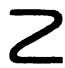
\includegraphics[keepaspectratio]{images/part001_42ca6df9.jpg}}

注记.—— 1) 设 E 与 E' 是 K 的两个可分闭包。若 K 不是可分封闭的，则存在多个 E 到 E' 上的 K-同构。因为此时 E 是 K 的非平凡伽罗瓦扩张，故存在异于恒等映射的 E 的 K-自同构（V，第 56 页，定理 1）。

2) 设 \(E\) 是 \(K\) 的一个代数可分扩张。若 \(K\) 的每个代数且可分的扩张都同构于 \(E\) 的一个子扩张，则 \(E\) 是 K 的一个可分闭包。因为若 \(E'\) 是 K 的一个可分闭包，则扩张 E 与 \(E'\) 中的每一个都同构于另一个的子扩张；因此 E 与 \(E'\) 是 K 的同构扩张（V，第 52 页，命题 1，a)）。

\subsection{有限次扩张的可分次数与不可分次数}

设 E 是 K 的有限次扩张，\(\Omega\) 是 K 的一个代数闭包。回顾（V，第 31 页），所谓 E 在 K 上的可分次数，记作 \([E:K]_{s}\) ，是指 E 到 \(\Omega\) 中的 K-同态的个数。

命题 15.——设 \(\mathbf{E}_s\) 是 \(\mathbf{K}\) 在 \(\mathbf{E}\) 中的相对可分闭包；则 \([\mathbf{E}:\mathbf{K}]_s = [\mathbf{E}_s:\mathbf{K}]\) .

域 \(\Omega\) 是完全的，且 \(E\) 是 \(p\) -根式的（在 \(E_s\) 上），这依据 \(V\) 第 44 页命题 13；因此命题 3（V，第 26 页）表明，\(E_s\) 到 \(\Omega\) 中的每个 K-同态都能以唯一方式延拓为 \(E\) 到 \(\Omega\) 中的 K-同态；于是我们有 \([E:K]_s = [E_s:K]_s\) 。由于 \(E_s\) 是 \(K\) 的有限次可分扩张，它是 \(K\) 上的平展代数；故 \([E_s:K]_s = [E_s:K]\) （由 \(V\) ，第 32 页，命题 4），结论得证。

沿用前面的记号，E 在 \(E_{s}\) 上的次数称为 E 在 K 上的不可分次数，记作 \([E:K]_{i}\) 。于是我们有

\[
[ \mathrm{E}: \mathrm{K} ] = [ \mathrm{E}: \mathrm{K} ] _ {s} \cdot [ \mathrm{E}: \mathrm{K} ] _ {i}\tag{1}
\]

由命题 15。

\pandocbounded{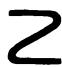
\includegraphics[keepaspectratio]{images/part001_fb7ec604.jpg}}

当 K 的特征为 0 时，有 \(E = E_{s}\) ，因此 \([E : K]_{s} = [E : K]\) 且 \([E : K]_{i} = 1\) 。若 K 的特征为 \(p \neq 0\) ，则数 \([E : K]_{i}\) 是 p 的幂，因为 E 在 \(E_{s}\) 上是 p-根式扩张（V，第 44 页，命题 13 及第 26 页，命题 4）。应当注意，\([E : K]_{i}\) 未必等于整除 \([E : K]\) 的 p 的最高次幂，也未必等于 E 在 K 中的相对 p-根式闭包的次数 \([E_{r} : K]\) （V，第 152 页，习题 3 和 2）。

命题 16.——设 \(\Omega\) 是 K 的一个扩张，E、F 是 \(\Omega\) 的两个子扩张，在 K 上次数有限。

\begin{enumerate}
\def\labelenumi{\alph{enumi})}
\item
  若 \(\mathrm{E} \subset \mathrm{F}\) ，则 \([\mathrm{F}:\mathrm{K}]_s = [\mathrm{F}:\mathrm{E}]_s \cdot [\mathrm{E}:\mathrm{K}]_s\) 且 \([\mathrm{F}:\mathrm{K}]_i = [\mathrm{F}:\mathrm{E}]_i \cdot [\mathrm{E}:\mathrm{K}]_i\) .
\item
  设 \(\mathbf{K}'\) 是 \(\Omega\) 的一个子扩张；则我们有
\end{enumerate}

\[
\left[ \mathrm{K} ^ {\prime} (\mathrm{E}): \mathrm{K} ^ {\prime} \right] _ {s} \leqslant \left[ \mathrm{E}: \mathrm{K} \right] _ {s} \quad \text{且} \quad \left[ \mathrm{K} ^ {\prime} (\mathrm{E}): \mathrm{K} ^ {\prime} \right] _ {i} \leqslant \left[ \mathrm{E}: \mathrm{K} \right] _ {i},
\]

且当 \(\mathbf{K}'\) 与 \(\mathbf{E}\) 在 \(\mathbf{K}\) 上线性不相交时等号成立。

\begin{enumerate}
\def\labelenumi{\alph{enumi})}
\setcounter{enumi}{2}
\tightlist
\item
  我们有 \([\mathrm{K}(\mathrm{E}\cup \mathrm{F}):\mathrm{K}]_s\leqslant [\mathrm{E}:\mathrm{K}]_s.\) \([\mathrm{F}:\mathrm{K}]_s\) 且 \([\mathrm{K}(\mathrm{E}\cup \mathrm{F}):\mathrm{K}]_i\leqslant [\mathrm{E}:\mathrm{K}]_i.\) \([\mathrm{F}:\mathrm{K}]_i\) ，且当 E 与 F 在 K 上线性不相交时等号成立。
\end{enumerate}

\(a\) 中关于可分次数的断言由 (9)（V，第 32 页）可得。由于 \([F:K] = [F:E].[E:K]\) ，关于不可分次数的断言由此及 (1) 得出。

由命题 13 的推论 1（V，第 44 页）及命题 15，我们有

\[
\left[ \mathrm{K} ^ {\prime} (\mathrm{E}): \mathrm{K} ^ {\prime} \right] _ {s} = \left[ \mathrm{K} ^ {\prime} \left(\mathrm{E} _ {s}\right): \mathrm{K} ^ {\prime} \right], \quad \left[ \mathrm{K} ^ {\prime} (\mathrm{E}): \mathrm{K} ^ {\prime} \right] _ {i} = \left[ \mathrm{F} ^ {\prime} (\mathrm{E}): \mathrm{K} ^ {\prime} \left(\mathrm{E} _ {s}\right) \right];\tag{2}
\]

当 \(K'\) 在 K 上与 E 线性不相交时，\(E_{s}\) 在 K 上与 \(K'\) 线性不相交，且 E 与 \(\mathrm{K}'(\mathrm{E}_{s})\) 在 \(E_{s}\) 上线性不相交（V，第 15 页，命题 8）。断言 b) 现由命题 5（V，第 14 页）得出。

由 a) 我们有 \([\mathbf{K}(\mathbf{E}\cup\mathbf{F}):\mathbf{K}]_{s}=[\mathbf{F}(\mathbf{E}):\mathbf{F}]_{s}\cdot[\mathbf{F}:\mathbf{K}]_{s}\) ；由 b) 我们有 \([\mathbf{F}(\mathbf{E}):\mathbf{F}]_{s}\leqslant[\mathbf{E}:\mathbf{K}]_{s}\) ，且当 E 与 F 在 K 上线性不相交时取等号。因此我们得到不等式 \([\mathbf{K}(\mathbf{E}\cup\mathbf{F}):\mathbf{K}]_{s}\leqslant[\mathbf{E}:\mathbf{K}]_{s}\cdot[\mathbf{F}:\mathbf{K}]_{s}\) ，且当 E 与 F 在 K 上线性不相交时取等号。c) 中关于不可分次数的断言可用类似的方式证明。

\section{范数与迹}

在本节中，K 表示一个域。

\subsection{回顾}

设 A 是 K 上次数为 n 的代数。对每个 \(x \in A\) ，用 \(L_{x}\) 表示线性映射 \(a \mapsto xa\) ，它把 A 映到自身。我们回顾（III，第 543 页），\(L_{x}\) 的迹称为 x 相对于 A 的迹，记作 \(\operatorname{Tr}_{\mathbf{A}/\mathbf{K}}(x)\) ；同样，\(L_{x}\) 的行列式称为 x 相对于 A 的范数，记作 \(\mathrm{N}_{\mathrm{A}/\mathrm{K}}(x)\) 。由 A 中 n 个元素构成的序列 \((x_{1}, \ldots, x_{n})\) 的判别式，按定义，是 \(\mathrm{D}_{\mathrm{A}/\mathrm{K}}(x_{1}, \ldots, x_{n})\) ，即矩阵 \((\operatorname{Tr}_{\mathrm{A}/\mathrm{K}}(x_{i}x_{j}))_{1 \leq i,j \leq n}\) 的行列式（III，第 549 页）。

设 \(\mathbf{K}'\) 是 \(\mathbf{K}\) 的一个扩张，令 \(\mathbf{A}' = \mathbf{A}_{(\mathbf{K}')}\) 为 \(\mathbf{K}'\) -代数，它由 \(\mathbf{A}\) 通过标量扩张得到。我们有公式

\[
\operatorname{Tr} _ {\mathrm{A} ^ {\prime} / \mathrm{K} ^ {\prime}} (1 \otimes x) = \operatorname{Tr} _ {\mathrm{A} / \mathrm{K}} (x). 1, \quad \mathrm{N} _ {\mathrm{A} ^ {\prime} / \mathrm{K} ^ {\prime}} (1 \otimes x) = \mathrm{N} _ {\mathrm{A} / \mathrm{K}} (x). 1\tag{1}
\]

对所有 \(x \in \mathbf{A}\) 成立（III，第 544 页）。对每个序列 \((x_1, \ldots, x_n)\) （其元素属于 \(\mathbf{A}\) ），我们有

\[
\mathrm{D} _ {\mathrm{A} ^ {\prime} / \mathrm{K} ^ {\prime}} (1 \otimes x _ {1}, \dots , 1 \otimes x _ {n}) = \mathrm{D} _ {\mathrm{A} / \mathrm{K}} (x _ {1}, \dots , x _ {n}). 1,\tag{2}
\]

这由第一个公式 (1) 得出。

\subsection{平展代数中的范数与迹}

设 A 是 K 上（有限）次数为 n 的平展代数。按定义，此时存在 K 的一个扩张 L 与 A 到 L 中的互不相同的同态 \(u_{1}, \ldots, u_{n}\) ，具有下列性质。

\begin{enumerate}
\def\labelenumi{\alph{enumi})}
\item
  \(\mathbf{A}\) 到 \(\mathbf{L}\) 中的每个同态都等于某个 \(u_{i}\) （V，第 29 页，推论）
\item
  存在 L-代数同构 \(u: \mathbf{A}_{(L)} \to L^n\) 使得
\end{enumerate}

\[
u (1 \otimes x) = \left(u _ {1} (x), \dots , u _ {n} (x)\right) \quad \text { for   all } \quad x \in A.
\]

此外，K 的每个代数闭扩张 L 都具有上述性质（V，第 30 页，命题 2）。

在以下的讨论中我们固定 \(L, u_1, \ldots, u_n\) 。设 \(x \in A\) ；我们将证明公式

\[
\operatorname{Tr} _ {\mathrm{A} / \mathrm{K}} (x) \cdot 1 = \sum_ {i = 1} ^ {n} u _ {i} (x), \quad \mathrm{N} _ {\mathrm{A} / \mathrm{K}} (x) \cdot 1 = \prod_ {i = 1} ^ {n} u _ {i} (x).\tag{3}
\]

设 \(v\) 为乘以 \(1 \otimes x\) 的映射，作用在 \(\mathbf{A}_{(L)}\) 上；相对于 \(\mathbf{A}_{(L)}\) 的那组基（即 \(u^{-1}\) 下 \(L^n\) 的典范基的像），线性映射 \(v\) 的矩阵是对角形的，其对角元为 \(u_1(x), \ldots, u_n(x)\) 。由此我们得出

\[
\operatorname{Tr} _ {\mathrm{A} _ {(\mathrm{L})} / \mathrm{L}} (1 \otimes x). 1 = \sum_ {i = 1} ^ {n} u _ {i} (x), \text { whence } \operatorname{Tr} _ {\mathrm{A} / \mathrm{K}} (x). 1 = \sum_ {i = 1} ^ {n} u _ {i} (x) \text { by } (1);
\]

范数的情形类似处理。

再设 \((x_{1},\ldots ,x_{n})\) 是由 A 的元素组成的序列，设 U 为矩阵

\[
\left(u _ {i} \left(x _ {j}\right)\right) _ {1 \leqslant i, j \leqslant n}
\]

并令 \((t_{ij}) = {}^t\mathrm{U} \cdot U\) 。由第一个公式 (3)，我们有

\[
\operatorname{Tr} _ {\mathrm{A} / \mathrm{K}} \left(x _ {i} x _ {j}\right) \cdot 1 = \sum_ {k = 1} ^ {n} u _ {k} \left(x _ {i} x _ {j}\right) = \sum_ {k = 1} ^ {n} u _ {k} \left(x _ {i}\right) u _ {k} \left(x _ {j}\right) = t _ {i j};
\]

取行列式，我们得到

\[
\mathrm{D} _ {\mathrm{A} / \mathrm{K}} (x _ {1}, \dots , x _ {n}) \cdot 1 = [ \det u _ {i} (x _ {j}) ] ^ {2}.\tag{4}
\]

命题 1.——设 A 是 K 上有限次的交换代数。则下列条件等价：

\begin{enumerate}
\def\labelenumi{\alph{enumi})}
\item
  代数 \(\mathbf{A}\) 是平展的。
\item
  存在 \(\mathbf{A}\) 的一组基，其判别式非零。
\item
  对 A 中每个 \(x \neq 0\) ，存在 A 中的 \(y\) 使得 \(\operatorname{Tr}_{\mathbf{A} / \mathbf{K}}(xy) \neq 0\) .
\end{enumerate}

此外，当这些条件满足时，A 的任何基的判别式都非零。

我们要证明：当假设 A 平展时，A 关于任意一组基 \((x_{1},\ldots,x_{n})\) （A 在 K 上的基）的判别式非零；这特别地确立了蕴含关系 \(a)\Rightarrow b)\) 。借助上述记号，由 (4)，只需证明矩阵 U 可逆，或等价地，证明线性方程组

\[
\sum_ {i = 1} ^ {n} \lambda_ {i} u _ {i} (x _ {j}) = 0 \quad (\text { for } 1 \leqslant j \leqslant n)\tag{5}
\]

在 L 中仅有解 \(\lambda_{1} = \cdots = \lambda_{n} = 0\) 。现在关系式 (5) 蕴含 \(\sum_{i=1}^{n} \lambda_{i} u_{i}(x) = 0\) （对所有 \(x \in \mathbf{A}\) ），从而 \(\lambda_{i} = 0\) （对 \(1 \leqslant i \leqslant n\) ），这依据的是

同态的线性无关性定理（V，第 27 页，定理 1）。

\(b)\) 与 \(c)\) 的等价性是下述一般引理的推论：

引理 1.——设 V 是 K 上有限维向量空间，B 是 V × V 上的一个双线性型。设 \((v_{1}, \ldots, v_{n})\) 是 V 在 K 上的一组基，并设 \(\Delta = \det B(v_{i}, v_{j})\) 。则 \(\Delta \neq 0\) 当且仅当：对 V 中每个 \(x \neq 0\) ，存在 V 中的 y 使得 \(B(x, y) \neq 0\) .

我们有 \(\Delta \neq 0\) 当且仅当线性方程组

\[
\sum_ {i = 1} ^ {n} \lambda_ {i} \mathrm{B} (v _ {i}, v _ {j}) = 0 \quad (1 \leqslant j \leqslant n)
\]

在 K 中只有解 \(\lambda_1 = \cdots = \lambda_n = 0\) 。若令 \(x = \sum_{i=1}^{n} \lambda_i v_i\) ，则上述方程组等价于 B \((x, v_j) = 0\) （对 \(1 \leqslant j \leqslant n\) ），也等价于——由于 \((v_1, \ldots, v_n)\) 是 V 在 K 上的一组基——B \((x, y) = 0\) 对所有 \(y \in V\) 成立，从而引理得证。

我们来证明条件 c) 蕴含 A 是既约的。设 x 是 A 中的幂零元；对任意 \(y \in A\) ，元素 xy 是幂零的，于是向量空间 A 的自同态 \(L_{xy}\) 是幂零的。而下述引理表明 \(\operatorname{Tr}(xy) = 0\) 对所有 \(y \in A\) 成立，从而在假设 c) 下有 x = 0。

引理 2.——设 V 是 K 上有限维向量空间，u 是 V 的一个幂零自同态，则 \(\operatorname{Tr}(u)=0\) .

对每个整数 \(n \geqslant 0\) ，令 \(V_n\) 为 \(u^n\) 的像。由于 \(u\) 是幂零的，存在整数 \(r \geqslant 0\) 使得 \(V_0 = V\) 、\(V_r = 0\) ，且 \(V_i \neq V_{i+1}\) （对 \(0 \leqslant i \leqslant r-1\) ）。令 \(d_i\) 为 \(V_{i-1}\) 的维数（对 \(1 \leqslant i \leqslant r\) ）。存在一组基 \((x_1, \ldots, x_d)\) （\(V\) 的），使得向量 \(x_j\) （满足 \(d - d_i < j \leqslant d\) ）构成 \(V_{i-1}\) 的一组基（对 \(1 \leqslant i \leqslant r\) ）。我们有 \(u(V_{i-1}) \subset V_i\) ，因此 \(u\) 在基 \((x_1, \ldots, x_d)\) 下的矩阵的对角元全为零。于是 \(\operatorname{Tr}(u) = 0\) ，引理得证。

最后我们证明 \(b)\) 蕴含 \(a)\) 。设 \((x_1, \ldots, x_n)\) 是 \(A\) 在 \(K\) 上的一组基，使得 \(D_{A/K}(x_1, \ldots, x_n) \neq 0\) 。设 \(K'\) 是 \(K\) 的一个扩张，\(A'\) 为 \(K'\) -代数（由 \(A\) 经标量扩张得到），且 \(x_i' = 1 \otimes x_i\) （对 \(1 \leqslant i \leqslant n\) ）。由公式 (2)（V，第 47 页），我们有 \(D_{A'/K'}(x_1', \ldots, x_n') \neq 0\) 。把前面的结果应用于 \(A'\) ，便知 \(A'\) 是既约的，从而代数 \(A\) 是平展的（V，第 34 页，定理 4）。

推论.——设 E 是 K 的有限次扩张。E 可分当且仅当存在 E 中的 a 使得 \(\operatorname{Tr}_{E/K}(a) \neq 0\) .

该条件由命题 1 知是必要的。反之，假设存在 \(a \in E\) 使得 \(\operatorname{Tr}_{E/K}(a) \neq 0\) 。给定 \(x \neq 0\) （\(E\) 中的），若令 \(y = ax^{-1}\) ，则 \(\operatorname{Tr}_{E/K}(xy) \neq 0\) 。于是命题 1 表明 \(E\) 是 \(K\) 上的一个平展代数，从而是 \(K\) 的可分扩张。

\subsection{有限次扩张中的范数与迹}

代数中的传递公式（III，第 548 页）在有限次扩张的情形下蕴含下述命题。

命题 2.——设 F 是 K 的有限次扩张，E 是 F 的一个子扩张。则对每个 \(x \in F\) 我们有

\[
\operatorname{Tr} _ {\mathrm{F} / \mathrm{K}} (x) = \operatorname{Tr} _ {\mathrm{E} / \mathrm{K}} (\operatorname{Tr} _ {\mathrm{F} / \mathrm{E}} (x))\tag{6}
\]

\[
\mathrm{N} _ {\mathrm{F} / \mathrm{K}} (x) = \mathrm{N} _ {\mathrm{E} / \mathrm{K}} (\mathrm{N} _ {\mathrm{F} / \mathrm{E}} (x))\tag{7}
\]

推论.——设 \(m = [F : E]\) ；则对每个 \(x \in E\) 我们有

\[
\operatorname{Tr} _ {\mathrm{F} / \mathrm{K}} (x) = m. \operatorname{Tr} _ {\mathrm{E} / \mathrm{K}} (x)\tag{8}
\]

\[
\mathrm{N} _ {\mathrm{F} / \mathrm{K}} (x) = \mathrm{N} _ {\mathrm{E} / \mathrm{K}} (x) ^ {m}\tag{9}
\]

命题 3.——设 E 是 K 的 n 次有限扩张，x 是 E 中在 K 上次数为 d 的元素。记 \(f(X) = X^d + \sum_{i=1}^{d} a_i X^{d-i}\) 为 x 在 K 上的极小多项式。则我们有

\[
\mathrm{Tr} _ {\mathrm{E/K}} (x) = - \frac {n}{d} a _ {1}\tag{10}
\]

\[
\mathrm{N} _ {\mathrm{E} / \mathrm{K}} (x) = ((- 1) ^ {d} a _ {d}) ^ {n / d} = (- 1) ^ {n} a _ {d} ^ {n / d}\tag{11}
\]

命题 3 直接由命题 2 的推论及下述引理得出：

引理 3.——设 R 是交换环，\(f(\mathbf{X}) = \mathbf{X}^d + \sum_{i=1}^{d} a_i \mathbf{X}^{d-i}\) 是 R{[}X{]} 中的一个首一多项式，A 是 R-代数 R{[}X{]}/(f)，x 是 X 在 A 中的剩余类。则 \(\operatorname{Tr}_{\mathrm{A/R}}(x) = -a_1\) 且 \(\mathrm{N}_{\mathrm{A/R}}(x) = (-1)^d a_d\) .

由该推论（IV，第 11 页），序列 \((1, x, \ldots, x^{d-1})\) 是 \(\mathbf{A}\) 的一组基；进一步我们有

\[
\begin{array}{r l} x \cdot 1 = x, & x \cdot x = x ^ {2}, \dots , x \cdot x ^ {d - 2} = x ^ {d - 1}, \\ & x \cdot x ^ {d - 1} = - a _ {d} \cdot 1 - a _ {d - 1} \cdot x - \dots - a _ {1} \cdot x ^ {d - 1}. \end{array}
\]

于是，相对于 A 的基 \((1, x, \ldots, x^{d-1})\) 表示乘以 x 的矩阵具有下述形式（为确定起见取 d = 5）：

\[
\left( \begin{array}{c c c c c} 0 & 0 & 0 & 0 & - a _ {5} \\ 1 & 0 & 0 & 0 & - a _ {4} \\ 0 & 1 & 0 & 0 & - a _ {3} \\ 0 & 0 & 1 & 0 & - a _ {2} \\ 0 & 0 & 0 & 1 & - a _ {1} \end{array} \right).
\]

这个矩阵的迹显然是 \(-a_{1}\) ；把行列式按第一行展开即可算得，于是我们得到

\[
(- 1) ^ {d - 1} (- a _ {d}) = (- 1) ^ {d} a _ {d}.
\]

在本小节其余部分，我们用 E 表示 K 的一个有限次扩张，并用 x 表示 E 中的一个元素。我们将指出在各种情形下如何计算 x 的范数与迹。

\begin{enumerate}
\def\labelenumi{\alph{enumi})}
\tightlist
\item
  可分扩张的情形：设 E 在 K 上是 n 次可分扩张，用 \(\Omega\) 表示 K 的一个代数闭包，用 \(\sigma_{1}, \ldots, \sigma_{n}\) 表示 E 到 \(\Omega\) 中的 n 个互不相同的 K-同态。由公式 (3)（V，第 48 页），我们在 \(\Omega\) 中有
\end{enumerate}

\[
\mathrm{Tr} _ {\mathrm{E} / \mathrm{K}} (x) = \sum_ {i = 1} ^ {n} \sigma_ {i} (x), \quad \mathrm{N} _ {\mathrm{E} / \mathrm{K}} (x) = \prod_ {i = 1} ^ {n} \sigma_ {i} (x).\tag{12}
\]

\begin{enumerate}
\def\labelenumi{\alph{enumi})}
\setcounter{enumi}{1}
\tightlist
\item
  p-根式扩张的情形：设 K 的特征为 p \textgreater{} 0 且扩张 E 是 p-根式的；存在整数 \(e \geqslant 0\) 使得 \([E : K] = p^{e}\) （V，第 26 页，命题 4）。若 f 是 x 在 K 上的高度，则 x 在 K 上的极小多项式是 \(X^{p^{f}} - x^{p^{f}}\) （V，第 24 页，命题 1）。由命题 3，我们有 \(\mathrm{N}_{\mathrm{E}/\mathrm{K}}(x) = (x^{p^{f}})^{p^{e}/p^{f}}\) ，从而
\end{enumerate}

\[
\mathrm{N} _ {\mathrm{E} / \mathrm{K}} (x) = x ^ {p ^ {e}} = x ^ {[ \mathrm{E}: \mathrm{K} ]}.\tag{13}
\]

对于迹，我们求得 \(\mathrm{Tr}_{\mathrm{E} / \mathrm{K}}(x) = -p^{e - f}a\) ，其中 \(a\) 是 \(\mathbf{X}^{p^f - 1}\) 在多项式 \(\mathbf{X}^{p^f} - x^{p^f}\) 中的系数；换言之，我们有

\[
\operatorname{Tr} _ {\mathrm{E} / \mathrm{K}} (x) = p ^ {e} \cdot x = [ \mathrm{E}: \mathrm{K} ] x = \left\{ \begin{array}{l l} x & \text { if } \quad [ \mathrm{E}: \mathrm{K} ] = 1 \\ 0 & \text { if } \quad [ \mathrm{E}: \mathrm{K} ] > 1. \end{array} \right.\tag{14}
\]

\begin{enumerate}
\def\labelenumi{\alph{enumi})}
\setcounter{enumi}{2}
\tightlist
\item
  一般情形：我们可以把范数与迹的计算总结为下述命题：
\end{enumerate}

命题 4.——设 p 是 K 的特征指数，E 是 K 的一个有限次扩张。设 \(\sigma_{1}, \ldots, \sigma_{n}\) 是 E 到 K 的一个代数闭包 \(\Omega\) 中的互不相同的 K-同态，并设 \(p^{e} = [E : K]_{i}\) 。对每个 \(x \in E\) ，我们在 \(\Omega\) 中有

\[
\operatorname{Tr} _ {\mathrm{E} / \mathrm{K}} (x) = p ^ {e} \cdot \sum_ {i = 1} ^ {n} \sigma_ {i} (x), \quad \mathrm{N} _ {\mathrm{E} / \mathrm{K}} (x) = \left(\prod_ {i = 1} ^ {n} \sigma_ {i} (x)\right) ^ {p ^ {e}}.\tag{15}
\]

设 \(E_s\) 是 K 在 E 中的相对可分闭包；则 \(E_s\) 是 K 的 n 次可分扩张，且 \(\sigma_1, \ldots, \sigma_n\) 诱导 \(E_s\) 到 \(\Omega\) 中的互不相同的 K-同态；此外，E 是 \(E_s\) 的次数为 \(p^e\) 的 p-根式扩张（V，第 44 页，命题 13 及第 46 页）。于是命题 4 由公式 (6)、(7)、(13)、(14) 及 (12) 得出。

\section{共轭元素与拟伽罗瓦扩张}

在本节中，K 表示一个域，\(\Omega\) 表示 K 的一个代数闭包。

\subsection{同构的扩张}

命题 1.——设 E 是 K 的一个扩张且包含在 Ω 中，u 是 E 到 Ω 中的一个 K-同态。

\begin{enumerate}
\def\labelenumi{\alph{enumi})}
\item
  若 \(u\) 将 \(E\) 映入 \(E\) 内，则 \(u\) 诱导出一个 \(K\) -自同构（\(E\) 的）。
\item
  存在 Ω 的一个 K-自同构 v 延拓 u。
\end{enumerate}

设 \(u(E) \subset E\) ；为证明 \(a)\) ，只需证明 \(u(E) = E\) 。设 \(x\) 是 \(E\) 中的元素，\(f\) 是 \(x\) 在 \(K\) 上的极小多项式，\(\Phi\) 是 \(f\) 在 \(E\) 中的根集。集合 \(\Phi\) 是有限的，\(u\) 作为 \(E\) 到 \(E\) 中的映射是单射，且我们有 \(u(\Phi) \subset \Phi\) ；因此 \(u(\Phi) = \Phi\) ，从而 \(x \in u(\Phi) \subset u(E)\) ；这表明 \(E = u(E)\) .

显然 \(\Omega\) 是 E 的、也是 \(u(E)\) 的代数闭包；因此（V，第 23 页，推论），同构 \(u\) （E 到 \(u(E)\) 上的）可延拓为一个同构 \(v\) （\(\Omega\) 到 \(\Omega\) 上的）.

\subsection{共轭扩张与共轭元素}

定义 1.——设 E 与 F 是包含在 Ω 中的 K 的两个扩张。若存在 Ω 的一个 K-自同构 u 使得 \(u(E) = F\) ，则称 E 与 F （在 Ω 中）共轭。Ω 的两个元素 x 与 y 称为在 K 上共轭，如果存在 Ω 的一个 K-自同构 u 使得 \(u(x) = y\) .

设 E 与 F 是包含在 \(\Omega\) 中的 K 的两个扩张。由命题 1，E 与 F 在 K 上共轭当且仅当它们是 K 的同构扩张。特别地，当存在 \(\Omega\) 的两个子集 A 与 B 使得 \(\mathrm{E} = \mathrm{K}(\mathrm{A})\) 且 \(\mathrm{F} = \mathrm{K}(\mathrm{B})\) ，并且存在 \(\Omega\) 的一个 K-自同构 u 使得 \(u(\mathrm{A}) = \mathrm{B}\) 时，即是如此。

关系 « x 与 y 在 K 上共轭 » 是 \(\Omega\) 中的一个等价关系；其等价类称为 \(\Omega\) 中的共轭类；它们是 \(\Omega\) 的全体 K-自同构构成的群在 \(\Omega\) 中的轨道。

命题 2.——设 \(x\) 与 \(y\) 是 \(\Omega\) 的两个元素。则下列条件等价：

\begin{enumerate}
\def\labelenumi{\alph{enumi})}
\item
  \(x\) 与 \(y\) 在 \(\mathbf{K}\) 上共轭。
\item
  存在一个 K-同构 \(v\) （\(\mathbf{K}(x)\) 到 \(\mathbf{K}(y)\) 上的），使得 \(v(x) = y\) 。
\item
  \(x\) 与 \(y\) 在 \(\mathbf{K}\) 上有相同的极小多项式。
\end{enumerate}

首先设 x 与 y 在 K 上共轭；设 u 是 \(\Omega\) 的一个 K-自同构，使得 \(u(x) = y\) ，并设 f 是 x 在 K 上的极小多项式。我们有

\[
f (y) = f (u (x)) = u (f (x)) = 0,
\]

且 \(f\) 是 \(\mathbf{K}[\mathbf{X}]\) 中的首一不可约多项式；因此（V，第 16 页，定理 1，c)），\(f\) 是 \(y\) 在 \(\mathbf{K}\) 上的极小多项式。于是 \(a)\) 蕴含 \(c)\) 。

现在设 x 与 y 在 K 上有相同的极小多项式 f。存在域 \(\mathrm{K}[\mathrm{X}]/(f)\) 到 \(\mathrm{K}(x)\) （相应地，到 \(\mathrm{K}(y)\) ）上的一个 K-同构，它把 X 模 (f) 的剩余类映到 x（相应地，y）（V，第 16 页，定理 1，b)）；因此存在 \(\mathrm{K}(x)\) 到 \(\mathrm{K}(y)\) 上的一个 K-同构 v，使得 \(v(x)=y\) 。故 c) 蕴含 b)。

最后，在假设 \(b\) ) 下，命题 1 蕴含存在一个 K-自同构 \(u\) （\(\Omega\) 的），它延拓 \(v\) ；于是我们有 \(u(x) = y\) ，从而 \(x\) 与 \(y\) 在 \(K\) 上共轭，故 \(b\) ) 蕴含 \(a\) )。

推论 1.——设 x 是 Ω 中的元素，在 K 上次数为 n，并设 f 是 x 在 K 上的极小多项式。x 在 K 上的共轭元是 f 在 Ω 中的根，其个数至多等于 n。

推论 2.——设 x 是 Ω 中的元素，在 K 上次数为 n。x 在 K 上可分当且仅当 x 在 Ω 中有 n 个共轭元；当此情形成立时，x 在 K 上的所有共轭元都在 K 上可分。

设 \(f\) 是 \(x\) 在 \(K\) 上的极小多项式；它的根是 \(x\) 在 \(K\) 上的共轭元，且这些根中的每一个都以 \(f\) 为其在 \(K\) 上的极小多项式。而 \(x\) 在 \(K\) 上可分当且仅当多项式 \(f\) 是可分的（V，第 39 页，命题 5），即当且仅当 \(f\) 有 \(n\) 个互不相同的根（在 \(\Omega\) 中）。推论 2 由此得证。

推论 3.——设 G 是 \(\Omega\) 的 K-自同构的群。G 在 \(\Omega\) 中的不变量集是相对 \(p\) -根式闭包（K 在 \(\Omega\) 中的）（V，第 25 页）。

换言之，一个元素 \(x\) （\(\Omega\) 的）是 \(p\) -根式的（在 \(\mathbf{K}\) 上）当且仅当它除自身外没有别的共轭元。

设 \(p\) 为特征指数，并设 \(x \in \Omega\) 。由 V 第 44 页命题 13，存在整数 \(m \geqslant 0\) 使得 \(y = x^{p^m}\) 在 K 上是代数且可分的。而 \(x\) 在 G 下不变当且仅当 \(y\) 在 G 下不变；由推论 2，这当且仅当 \(y\) 在 K 上次数为 1，即 \(y \in K\) 。由此推论立即可得。

\subsection{拟伽罗瓦扩张}

定义 2.——设 E 是 K 的一个扩张。若 E 是代数的，并且 K{[}X{]} 中在 E 里至少有一个根的每个不可约多项式都在 E{[}X{]} 中分解为一些 1 次多项式（未必互异）之积，则称 E （在 K 上）是拟伽罗瓦的或正规的。

若 E 是 K 的一个代数闭包，则它是 K 的拟伽罗瓦扩张；因为命题 1 的条件 (AC)（V，第 19 页）断言 E{[}X{]} 中的每个非常数多项式都是一些 1 次多项式之积。

命题 3.——设 E 是包含在 Ω 中的 K 的一个扩张。则下列条件等价：

\begin{enumerate}
\def\labelenumi{\alph{enumi})}
\item
  E 是 K 的一个拟伽罗瓦扩张。
\item
  对每个 \(x \in \mathbf{E}\) ，\(x\) 在 \(\mathbf{K}\) 上的、位于 \(\Omega\) 中的共轭元都属于 \(\mathbf{E}\) 。
\item
  \(\Omega\) 的每个 K-自同构都把域 E 映到其自身内。
\item
  E 到 \(\Omega\) 中的每个 K-同态都把 E 映到其自身内。
\item
  E 是 \(\Omega\) 中一族非常数多项式 \((f_i)_{i\in I}\) （K{[}X{]} 中的）所确定的分裂扩张（V，第 24 页，注 3）。
\end{enumerate}

c) 与 d) 的等价性源于这样的事实：E 到 \(\Omega\) 中的每个 K-同态都由 \(\Omega\) 的一个 K-自同构诱导（V，第 52 页，命题 1）。

按定义，拟伽罗瓦扩张是其元素的（在 K 上的）极小多项式所成族的分裂域，故 \(a\) 蕴含 \(e\) )。在假设 \(e\) 下，设 \(u\) 是 \(\Omega\) 的一个自同构；对每个 \(i \in I\) ，\(u\) 置换根集 \(\mathbf{R}_i\) （\(f_i\) 的），且由于 \(\mathbf{E} = \mathbf{K}\left(\bigcup_{i \in I} \mathbf{R}_i\right)\) ，我们有 \(u(\mathbf{E}) = \mathbf{E}\) ；于是 \(e\) 蕴含 \(c\) 。

共轭元素的定义表明 \(c)\) 蕴含 \(b)\) 。最后假设 \(b)\) 成立；设 \(f\) 是 \(K[X]\) 中的一个首一不可约多项式，它至少有一个根 \(x\) （\(E\) 中的）；由于 \(\Omega\) 是代数闭的，存在元素 \(a_k\) （\(\Omega\) 的，\(1 \leqslant k \leqslant n\) ）使得 \(f(x) = \prod_{k=1}^{n} (X - a_k)\) ，又由于 \(a_k\) 是 \(x\) 在 K 上的共轭元（V，第 53 页，推论 1），由假设它们属于 E。于是我们证明了 b) 蕴含 a)。

推论 1.——包含在 Ω 中的 K 的扩张 E 是拟伽罗瓦的，当且仅当它与它在 K 上的所有共轭相同。

这由命题 1 的 a)（V，第 52 页）以及命题 3 中条件 \(a\) 与 \(c\) 的等价性得出。

推论 2.——设 E 与 F 是 K 的两个代数扩张，且 \(E \subset F\) 。若 F 在 K 上是拟伽罗瓦的，则它在 E 上也是拟伽罗瓦的。

我们可以假设 \(F \subset \Omega\) 。设 u 是 \(\Omega\) 的一个 E-自同构。由于 u 是 \(\Omega\) 的 K-自同构且 F 在 K 上拟伽罗瓦，我们有 \(u(F) = F\) ，因此 F 在 E 上是拟伽罗瓦的。

推论 3.——设 N 是包含在 \(\Omega\) 中的 K 的一个拟伽罗瓦扩张，E 是 N 的一个子扩张。设 u 是 E 到 \(\Omega\) 中的一个 K-同态；则 \(u(E) \subset N\) ，且存在 N 的一个 K-自同构 v，它在 E 上诱导 u。

设 w 是 \(\Omega\) 的一个延拓 u 的 K-自同构（V，第 52 页，命题 1）；由于 N 在 K 上拟伽罗瓦，我们有 \(w(\mathbf{N}) = \mathbf{N}\) ，从而 \(w(\mathbf{E}) \subset \mathbf{N}\) ，于是 w 诱导出 N 的一个 K-自同构 v。

推论 4.——设 E' 是 K 的一个扩张，E 与 K' 是 E' 的两个子扩张。假设 E 在 K 上是拟伽罗瓦的且 E' = K'(E) ；则 E' 在 K' 上是拟伽罗瓦的。

设 \((f_i)_{i\in I}\) 是 \(\mathbf{K}[\mathbf{X}]\) 中的一族非常数多项式，它们在 \(\mathbf{K}\) 上的分裂域是 E。则显然 \(\mathbf{E}'\) 是该族 \((f_i)_{i\in I}\) 在 \(\mathbf{K}'\) 上的分裂域，故它在 \(\mathbf{K}'\) 上是拟伽罗瓦的。

注.——1) 设 F 是 K 的一个扩张，E 是 F 的一个子扩张，且假设 E 在 K 上是拟伽罗瓦的。我们来证明 F 的每个 K-自同构 u 都保持 E 不变。设 \(x \in E\) ，f 是 x 在 K 上的极小多项式。由于 E 在 K 上拟伽罗瓦，存在 \(a_{1}, \ldots, a_{n} \in E\) 使得 \(f(\mathbf{X}) = \prod(\mathbf{X} - a_{i})\) ；我们有 \(f(u(x)) = u(f(x)) = 0\) ，故 \(u(x)\) 是某个 \(a_{i}\) ，从而属于 E。我们已证明 \(u(\mathrm{E}) \subset \mathrm{E}\) ，再由 V 第 52 页命题 1 即得 \(u(\mathrm{E}) = \mathrm{E}\) 。

\pandocbounded{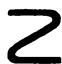
\includegraphics[keepaspectratio]{images/part001_36e9f8fa.jpg}}

\begin{enumerate}
\def\labelenumi{\arabic{enumi})}
\setcounter{enumi}{1}
\item
  设 E 是 K 的一个拟伽罗瓦扩张，F 是 E 的一个拟伽罗瓦扩张；F 在 K 上未必是拟伽罗瓦的（V，第 153 页，例 1）。原因如下：设 u 是 \(\Omega\) 的一个 K-自同构；我们有 \(u(E) = E\) ，但若 f 是 F 的元素 x 在 E 上的极小多项式，它在 u 下未必不变；因此 \(u(x)\) 未必与 x 在 E 上共轭，从而未必属于 F。在这种情形，F 与 \(u(F)\) 是 E 的两个不同的拟伽罗瓦扩张，它们是 K-同构的但不是 E-同构的。
\item
  设 E 是 K 的一个代数扩张，x、y 是 E 的两个元素。若存在 E 的一个 K-自同构把 x 映到 y，则 x 与 y 在 K 上有相同的极小多项式，从而由命题 2（V，第 52 页）在 K 上共轭。若 E 是拟伽罗瓦的，则逆命题成立，因为 \(\Omega\) 的每个 K-自同构都诱导 E 的一个 K-自同构。E 是拟伽罗瓦的这一假设并非多余，如下例所示：设 K = Q，\(\Omega\) 为全体代数数构成的域；令 \(E = \Omega \cap R\) 。可以证明（V，第 153 页，例 2），E 的每个自同构都是恒等映射，且 \(\sqrt{2}\) 与 \(-\sqrt{2}\) 是 E 中在 Q 上共轭的元素。
\end{enumerate}

\subsection{由集合生成的拟伽罗瓦扩张}

命题 4.——设 \((\mathbf{N}_i)_{i\in I}\) 是包含在 \(\Omega\) 中的 K 的一族拟伽罗瓦扩张。令 \(\mathbf{N} = \bigcap_{i\in I}\mathbf{N}_i\) 且 \(\mathbf{M} = \mathbf{K}\left(\bigcup_{i\in I}\mathbf{N}_i\right)\) ；则扩张 N 与 M

在 K 上都是拟伽罗瓦的。

设 \(u\) 是 \(\Omega\) 的一个 K-自同构。我们有 \(u(\mathbf{N}_i) = \mathbf{N}_i\) （对所有 \(i \in I\) ），由此得到等式 \(u(\mathbf{N}) = \mathbf{N}\) 与 \(u(\mathbf{M}) = \mathbf{M}\) ；于是命题由推论 1（V，第 54 页）得出。

设 A 是由 \(\Omega\) 的元素组成的一个集合，B 是由 \(\Omega\) 中与 A 的元素共轭的元素组成的集合；换句话说，若 G 是 \(\Omega\) 的 K-自同构的群，则我们有 \(\mathbf{B} = \bigcup_{u \in G} u(\mathbf{A})\) 。对每个 \(u \in G\) 我们有

\(u(B) = B\) ，从而 \(u(K(B)) = K(B)\) 。因此 \(K(B)\) 是 K 的一个包含 A 的拟伽罗瓦扩张，且显然 K 的每个包含 A 的拟伽罗瓦扩张 N 都包含 B，从而包含 \(K(B)\) 。我们称 \(K(B)\) 为由 A 生成的拟伽罗瓦扩张。这一定义特别适用于 A 是 K 的扩张的情形。

下述命题直接由前面的注得到。

命题 5.——设 E 是包含在 Ω 中的 K 的一个扩张，N 是由 E 生成的拟伽罗瓦扩张。若 A 是 Ω 的一个子集使得 E = K(A)，则 N = K(B)，其中 B 是 Ω 中与 A 的某个元素共轭的元素组成的集合。

推论 1.——若 E 是 K 的有限次扩张，则由 E 生成的 K 的拟伽罗瓦扩张 N 在 K 上是有限次的。

因为我们有 \(E = K(A)\) ，其中 A 是有限的，从而 A 的元素的共轭元所成的集 B 是有限的，于是推论由定理 2（V，第 18 页）得出。

推论 2.——K 的每个拟伽罗瓦扩张 N 都是 N 的在 K 上有限的拟伽罗瓦子扩张之并。

设 \(x \in \mathbb{N}\) ，并设 \(\mathbf{N}_x\) 是 \(\mathbf{K}\) 的一个拟伽罗瓦扩张（由 \(\{x\}\) 生成的）。由于 \(\mathbf{K}(x)\) 在 \(\mathbf{K}\) 上是有限次的，\(\mathbf{N}_x\) 亦然（推论 1），且我们有 \(x \in \mathbf{N}_x\) .

\section{伽罗瓦扩张}

在本节中，K 表示一个域。

\subsection{伽罗瓦扩张的定义}

定理 1.——设 N 是 K 的一个代数扩张，\(\Gamma\) 是 N 的 K-自同构的群。则下列断言等价：

\begin{enumerate}
\def\labelenumi{\alph{enumi})}
\item
  \(\mathbf{N}\) 中在 \(\Gamma\) 下不变的每个元素都属于 \(\mathbf{K}\) 在 \(\mathbf{N}\) 中的像。
\item
  N 是 K 的一个可分拟伽罗瓦扩张。
\item
  对每个 \(x \in \mathbf{N}\) ，\(x\) 在 \(\mathbf{K}\) 上的极小多项式在 \(\mathbf{N}[\mathbf{X}]\) 中分解为一些互异的 1 次多项式之积。
\end{enumerate}

b) 与 c) 的等价性由命题 6 的推论（V，第 40 页）及拟伽罗瓦扩张的定义（V，第 53 页，定义 2）得出。我们把 K 与它在 N 中的典范像等同起来。

\(a) \Rightarrow c)\) ：设 K 是 \(\Gamma\) 的不变量域。设 \(x \in \mathbf{N}\) ，其在 K 上的极小多项式为 \(f\) ，并设 A 为 \(f\) 在 N 中的全体根组成的集。令

\[
g (\mathbf {X}) = \prod_ {y \in \mathsf {A}} (\mathbf {X} - y).
\]

每个自同构 \(\sigma \in \Gamma\) 都诱导 \(\mathbf{A}\) 的一个置换，从而保持多项式 \(g \in \mathbf{N}[\mathbf{X}]\) 的系数不变。于是我们有 \(g \in \mathbf{K}[\mathbf{X}]\) ，且由于 \(g(x) = 0\) ，多项式 \(g\) 是 \(f\) 在 \(\mathbf{K}[\mathbf{X}]\) 中的倍式（V，第 16 页，定理 1）。再者，\(f\) 与 \(g\) 都是首一的，且 \(g\) 整除 \(f\) （IV，第 16 页，命题 5）；从而 \(f = g\) ，这意味着极小多项式 \(f\) （\(x\) 的，在 \(\mathbf{K}\) 上的）在 \(\mathbf{N}[\mathbf{X}]\) 中是一些互异的 1 次多项式之积。

\(c) \Rightarrow a)\) ：设 \(x\) 是 \(\mathbf{N}\) 中不属于 \(\mathbf{K}\) 的元素。用 \(\Omega\) 表示 \(\mathbf{K}\) 的一个把 \(\mathbf{N}\) 作为子扩张包含在内的代数闭包（V，第 23 页，定理 2）。设 \(f\) 是 \(x\) 在 \(\mathbf{K}\) 上的极小多项式，由假设它的次数 \(\geqslant 2\) ，并设 \(\mathbf{A}\) 是 \(f(\mathbf{X})\) 在 \(\mathbf{N}\) 中的根集。若条件 \(c)\) 成立，我们有 \(f(\mathbf{X}) = \prod_{y \in \mathbf{A}} (\mathbf{X} - y)\) ，于是

（V，第 53 页，推论 1）A 是 \(x\) 在 \(\Omega\) 中的共轭元之集。由于 \(f\) 的次数 \(\geqslant 2\) ，A 中存在元素 \(y \neq x\) ，从而存在一个 K-自同构 \(u\) （\(\Omega\) 的）使得 \(u(x) = y\) 。而在假设 \(c\) ) 下，K 的扩张 N 是拟伽罗瓦的，故 \(u(N) = N\) （V，第 54 页，推论 1）；由此 \(u\) 诱导 N 的一个 K-自同构 \(\sigma\) ，使得 \(\sigma(x) = y \neq x\) ，因此 K 是 \(\Gamma\) 的不变量域。

定义 1.——K 的扩张 N 称为伽罗瓦扩张，如果它是代数的且满足定理 1 的等价条件 a)、b)、c)。

设 N 是一个域，\(\Gamma\) 是 N 的一个自同构群，\(N_{0}\) 是 \(\Gamma\) 的不变量域。当 N 在 \(N_{0}\) 上代数时，它是 \(N_{0}\) 的伽罗瓦扩张。但情形未必总是如此：例如，设 K 是无限域，取 N 为有理分式域 \(\mathrm{K}(\mathrm{X})\) ；对每个 \(a \in K\) ，令 \(\sigma_{a}\) 为 \(\mathrm{K}(\mathrm{X})\) 的把 \(f(\mathrm{X})\) 映到 \(f(\mathrm{X} + a)\) 的自同构。所有 \(\sigma_{a}\) 组成的集是 \(\mathrm{K}(\mathrm{X})\) 的一个自同构群，其不变量域容易看出是 K；然而 \(\mathrm{K}(\mathrm{X})\) 在 K 上不是代数的。

设 \(\Omega\) 是 K 的一个代数闭包，设 A 表示由 \(\Omega\) 中在 K 上可分的元素组成的集，B 表示 A 的元素在 K 上的共轭元组成的集。则 B 由在 K 上代数且可分的元素组成。因此（V，第 39 页，命题 6 及第 56 页，命题 5）域 K(B) 是 K 的可分拟伽罗瓦扩张；换句话说，由 A 生成的拟伽罗瓦扩张（V，第 55 页）是 K 的伽罗瓦扩张；我们也称它为由 \(\Omega\) 的子集 A 生成的 K 的伽罗瓦扩张。

特别地，\(\Omega\) 中一族在 K 上可分的多项式的分裂域，以及 K 的可分闭包，都是 K 的伽罗瓦扩张。

命题 1.——设 N 是 K 的一个扩张，\((\mathbf{N}_{i})_{i\in I}\) 是 N 的子扩张的一个非空族。令 \(E=\bigcap_{i\in I}N_{i}\) 且 \(F=K\left(\bigcup_{i\in I}N_{i}\right)\) 。若所有扩张

\(N_{i}\) 在 K 上都是伽罗瓦的，则 E 与 F 亦然。

首先，E 在 K 上是代数且可分的（V，第 36 页，命题 1），对 F 同样成立（V，第 41 页，命题 8）。此外，由命题 4（V，第 55 页），E 与 F 在 K 上都是拟伽罗瓦的。

命题 2.——设 N 是 K 的一个伽罗瓦扩张，E 是 N 的一个子扩张，且在 K 上次数有限。存在 N 的一个包含 E 的子扩张 F，它在 K 上是伽罗瓦的且次数有限。

由于 N 在 K 上拟伽罗瓦，V 第 56 页推论 1 证明了存在 N 的一个包含 E 且在 K 上次数有限的拟伽罗瓦子扩张 F。由于 N 在 K 上可分，对 F 同样成立（V，第 36 页，命题 1），故 F 在 K 上是伽罗瓦的。

命题 2 蕴含下述结果：设 \(\Omega\) 是 K 的一个代数闭包，\(E_1, \ldots, E_n\) 是包含在 \(\Omega\) 中的 K 的有限次可分代数扩张。则存在 K 的一个有限次伽罗瓦扩张 N，它包含在 \(\Omega\) 中且包含 \(E_1, \ldots, E_n\) .

\subsection{伽罗瓦群}

定义 2.——设 N 是域 K 的一个伽罗瓦扩张。N 的全体 K-自同构组成的群称为 N 在 K 上的伽罗瓦群，记作 Gal(N/K)。

设 N 是 K 的一个有限伽罗瓦扩张。则 N 是 K 的有限可分拟伽罗瓦扩张。因此（V，第 32 页，命题 4 及 V，第 54 页，命题 3），Gal(N/K) 的阶等于 {[}N : K{]}。我们稍后将证明：若 N 是 K 的伽罗瓦扩张且 Gal(N/K) 是有限的，则 N 在 K 上次数有限（V，第 66 页，定理 3）。

设 \(\Omega\) 是 K 的一个代数闭扩张，设 A 是一个可分多项式在 \(\Omega\) 中的根集，该多项式记作 \(f \in \mathbf{K}[\mathbf{X}]\) 。则域 \(\mathbf{N} = \mathbf{K}(\mathbf{A})\) 是 K 的伽罗瓦扩张。显然，N 的每个 K-自同构都保持 A 稳定，且由于 A 在 K 上生成 N，映射 \(\sigma \mapsto \sigma | \mathbf{A}\) 是 \(\operatorname{Gal}(\mathbf{N} / \mathbf{K})\) 到一个子群 \(\Gamma\) （集 A 的对称群 \(\mathfrak{S}_{\mathbf{A}}\) 的）上的同构，该子群称为多项式 \(f\) 的伽罗瓦群。由注 3（V，第 55 页）可知，若 \(x\) 与 \(y\) 属于 A，则下列性质等价：

\begin{enumerate}
\def\labelenumi{\alph{enumi})}
\item
  \(x\) 与 \(y\) 在 \(\mathbf{K}\) 上共轭，
\item
  \(x\) 与 \(y\) 属于 \(\Gamma\) 作用下的同一轨道，
\item
  \(x\) 与 \(y\) 是 \(f\) 的同一个不可约因子的根。
\end{enumerate}

特别地，\(f\) 不可约当且仅当 \(\mathbf{A}\) 非空且 \(\Gamma\) 传递地作用于 \(\mathbf{A}\) 上。

例.——1) 设 K 的特征异于 2，N 是 K 的一个二次扩张。若 \(x \in \mathbf{N} - \mathbf{K}\) ，则我们有 \(\mathbf{N} = \mathbf{K}(x)\) ，且 \(x\) 在 K 上的极小多项式形如 \(f(\mathbf{X}) = \mathbf{X}^2 - a\mathbf{X} + b\) ，其中 \(a, b \in \mathbf{K}\) 。于是我们有 \(f(\mathbf{X}) = (\mathbf{X} - x)(\mathbf{X} - y)\) ，其中 \(y = a - x\) ，故 \(y\) 与 \(x\) 共轭；由于 \(f(\mathbf{X})\) 可分，扩张 N 是伽罗瓦的。群 \(\operatorname{Gal}(\mathbf{N}/\mathbf{K})\) 有两个元素，它们诱导集 \(\{x, y\}\) 的两个置换。

2) 设 \(f = \mathbf{X}^3 + \mathbf{X}^2 - 2\mathbf{X} - 1 \in \mathbf{Q}[\mathbf{X}]\) 。多项式 \(f\) 是不可约的；因为否则它将有一个根 \(x \in \mathbf{Q}\) ；把 \(x = a / b\) 写成 \(a, b \in \mathbf{Z}\) 且 \(a\) 与 \(b\) 互素的形式，我们将得到 \(a(a^2 + ab - 2b^2) = b^3\) 与 \(a^3 = b(b^2 + 2ab - a^2)\) ；但这蕴含 \(a\) 整除 \(b\) 且 \(b\) 整除 \(a\) ，从而 \(x = \pm 1\) ，这是不可能的。令 \(\xi = e^{2\pi i / 7} \in \mathbf{C}\) ；则多项式 \(f\) 以 \(\alpha = \xi + \xi^{-1}, \beta = \xi^2 + \xi^{-2}, \gamma = \xi^3 + \xi^{-3}\) 为根。我们有 \(\beta = \alpha^2 - 2\) 与 \(\gamma = \alpha^3 - 3\alpha\) ，故扩张 \(\mathbf{Q}(\alpha)\) 在 \(\mathbf{Q}\) 上是伽罗瓦的。\(\mathbf{Q}(\alpha)\) 在 \(\mathbf{Q}\) 上的伽罗瓦群是 3 阶循环群，由一个元素 \(\sigma\) 生成，使得 \(\sigma(\alpha) = \beta, \sigma(\beta) = \gamma, \sigma(\gamma) = \alpha.\)

\begin{enumerate}
\def\labelenumi{\arabic{enumi})}
\setcounter{enumi}{2}
\item
  设 K = Q 并取 \(f = X^{3} - 2\) 。利用整数分解为素因子之积（I，第 51 页），我们容易看出 2 不是 Q 中元素的立方。因此多项式 f 不可约，因为否则它在 Q 中将有一个根。设 \(A = \{x_{1}, x_{2}, x_{3}\}\) 为 f 在 \(\Omega\) 中的根集，\(\Gamma\) 为 f 的伽罗瓦群。它传递地作用于 A 上；故其阶可被 3 整除。另一方面，商 \(j = \frac{x_{2}}{x_{1}}\) 异于 1 且我们有 \(j^{3} = 1\) 。故 j 满足关系式 \(j^{2} + j + 1 = 0\) ；而多项式 \(T^{2} + T + 1 = \left(T + \frac{1}{2}\right)^{2} + \frac{3}{4}\) 在 Q 中没有根，这表明（例 1）\([Q(j): Q] = 2\) 。于是 \([N: Q]\) 可被 2 整除，从而 \(\Gamma\) 的阶可被 6 整除。由于 \(\Gamma\) 包含在 6 阶的群 \(S_{A}\) 之中，我们有 \(\Gamma = S_{A}\) .
\item
  设 K 的特征为 \(p \neq 0\) ，令 \(\mathrm{K}(\mathrm{T})\) 为有理分式域，\(U = T^{p} - T\) 。令 \(E = K[U]\) 且 \(F = K[T]\) ，则多项式 \(f(X) = X^{p} - X - U\) （\(E[X]\) 中的）在 F 中有根 \(T, T + 1, \ldots, T + p - 1\) 。设 \(\sigma\) 为 F 的使 \(\sigma(T) = T + 1\) 的 K-自同构。我们有 \(\sigma^{i}(T) = T + i\) 及 \(\sigma(U) = U\) 。群 \(G = \{1, \sigma, \ldots, \sigma^{p-1}\}\) 是 p 阶循环群，其不变量域包含 E；由于 \([F: E] \leqslant p\) ，戴德金定理（V，第 27 页，推论 2）蕴含 E 是 G 的不变量域且 \([F: E] = p\) 。于是多项式 f 在 \(E[X]\) 中不可约；E 的扩张 F 是伽罗瓦的，其伽罗瓦群 G 是 p 阶循环群，而群 \(\Gamma\) 是 T、\(T + 1, \ldots, T + p - 1\) 的循环置换所成的群。
\end{enumerate}

关于此例的推广，见 V，第 93 页，例 2。

\begin{enumerate}
\def\labelenumi{\arabic{enumi})}
\setcounter{enumi}{4}
\tightlist
\item
  设 \(\mathbf{F} = \mathbf{K}(\mathbf{X}_1, \ldots, \mathbf{X}_n)\) 是 \(n\) 个未定元 \(\mathbf{X}_1, \ldots, \mathbf{X}_n\) 在 \(\mathbf{K}\) 上的有理分式域。令
\end{enumerate}

\[
s _ {k} = \sum_ {1 \leqslant i _ {1} <   \dots <   i _ {k} \leqslant n} X _ {i _ {1}} \dots X _ {i _ {k}}
\]

其中 \(1 \leqslant k \leqslant n\) ，并令 \(\mathrm{E} = \mathrm{K}(s_1, \ldots, s_n)\) ；我们用 \(f(\mathrm{T})\) 表示多项式

\[
\mathrm{T} ^ {n} - s _ {1} \mathrm{T} ^ {n - 1} + \dots + (- 1) ^ {n} s _ {n}.
\]

我们有 \(f(\mathrm{T}) = \prod_{i=1}^{n} (\mathrm{T} - \mathrm{X}_i)\) ，故 \(\mathbf{F}\) 是可分多项式 \(f(\mathrm{T}) \in \mathrm{E}[\mathrm{T}]\) 的一个分裂域。进而，对每个置换 \(\sigma \in \mathfrak{S}_n\) ，存在唯一一个 \(\mathbf{K}\) -自同构 \(h_\sigma\) （\(\mathbf{F}\) 的），使得 \(h_\sigma(\mathrm{X}_i) = \mathrm{X}_{\sigma(i)}\) （对 \(1 \leqslant i \leqslant n\) ）；我们有 \(h_\sigma(s_k) = s_k\) （对 \(1 \leqslant k \leqslant n\) ），故 \(h_\sigma\) 是 \(\mathbf{F}\) 的一个 E-自同构。换言之，\(\mathbf{F}\) 是 \(\mathbf{E}\) 的伽罗瓦扩张，且在根集 \(\{\mathbf{X}_1, ..., \mathbf{X}_n\}\) （\(f(\mathrm{T})\) 的）上的限制定义了 \(\operatorname{Gal}(\mathrm{F}/\mathrm{E})\) 到群 \(\mathfrak{S}_n\) 上的一个同构。特别地，\(\mathbf{E}\) 由满足下式的有理分式 \(f\) 组成：

\[
f \left(\mathrm{X} _ {\sigma (1)}, \dots , \mathrm{X} _ {\sigma (n)}\right) = f \left(\mathrm{X} _ {1}, \dots , \mathrm{X} _ {n}\right)
\]

（对每个 \(\sigma \in \mathfrak{S}_n\) ；参看 IV，第 67 页，推论。）

\begin{enumerate}
\def\labelenumi{\arabic{enumi})}
\setcounter{enumi}{5}
\tightlist
\item
  设 \(f\) 是次数 \(> 0\) 的首一多项式，且 \(K\) 的特征 \(\neq 2\) 。在 \(A\) 上定义一个全序，记作 \(\leqslant\) ，并令 \(\delta(f) = \prod_{\alpha < \beta} (\beta - \alpha)\) ，
\end{enumerate}

\((\alpha, \beta) \in \mathbf{A} \times \mathbf{A}\) ，并对每个 \(\sigma \in \mathfrak{S}_{\mathbf{A}}\) 令 \(\delta_{\sigma}(f) = \prod_{\alpha < \beta} (\sigma(\beta) - \sigma(\alpha))\) 。我们有

\(\delta_{\sigma}(f) = \varepsilon(\sigma)\ \delta(f)\) ，其中 \(\varepsilon(\sigma)\) 是 \(\sigma\) 的符号（I，第 64 页），且 \(\delta(f) \neq 0\) 。对每个 \(\tau \in \operatorname{Gal}(\mathbf{N}/\mathbf{K})\) ，我们有 \(\tau(\delta(f)) = \delta_{\tau|_{\mathbf{A}}}(f)\) 。因此 \(\Gamma\) 包含在交错群 \(\mathfrak{A}_{\mathbf{A}}\) 中当且仅当 \(\delta(f) \in \mathbf{K}\) 。此外，\(\delta(f)^2 = \prod_{\alpha < \beta} (\beta - \alpha)^2 =\)

\(d(f)\) 是多项式 \(f\) 的判别式（IV，第 81 页）。因此 \(\Gamma \subset \mathfrak{A}_{\mathbf{A}}\) 当且仅当 \(d(f)\) 是 \(\mathbf{K}\) 中某个元素的平方。于是在例 2 中我们有 \(d(f) = 49 = 7^2\) ，而在例 3 中 \(d(f) = -108\) （IV，第 85 页）。

设 N 是 K 的一个伽罗瓦扩张，L 是 N 的一个在 K 上伽罗瓦的子扩张。N 的每个 K-自同构 \(\sigma\) 都诱导 L 的一个 K-自同构 \(\sigma_{L}\) （V，第 55 页，注 1）。因此映射 \(\sigma \mapsto \sigma_{L}\) 是 \(\operatorname{Gal}(N/K)\) 到 \(\operatorname{Gal}(L/K)\) 中的同态，称为限制同态。

命题 3.——Gal(N/K) 到 Gal(L/K) 的限制同态是满射。

更一般地，考虑 N 的两个子扩张 L 与 L'，以及 L 到 L' 上的一个 K-同构 u。选取 K 的一个把 N 作为子扩张包含在内的代数闭包 \(\Omega\) （V，第 23 页，定理 2）。存在 \(\Omega\) 的一个在 L 上与 u 一致的 K-自同构 v（V，第 52 页，命题 1），且由于 N 是 K 的拟伽罗瓦扩张，v 诱导 N 的一个 K-自同构 \(\sigma\) （V，第 55 页，注 1）。换言之，Gal(N/K) 中的元素 \(\sigma\) 在 L 上与 u 一致。

\subsection{伽罗瓦群的拓扑}

设 N 是 K 的一个伽罗瓦扩张，\(\Gamma\) 是 N 在 K 上的伽罗瓦群。我们给 N 赋以离散拓扑，给 N 到自身的全体映射组成的集 \(N^{N}\) 赋以诸因子的离散拓扑的积拓扑（« N 中简单收敛拓扑 »），并给群 \(\Gamma\) 赋以由 \(N^{N}\) 诱导的拓扑。

设 \(\Lambda\) 为 \(\mathbf{N}\) 的在 \(\mathbf{K}\) 上次数有限的全体子扩张组成的集。对 \(\sigma \in \Gamma\) 与 \(\mathrm{E} \in \Lambda\) ，我们用 \(\mathrm{U}_{\mathrm{E}}(\sigma)\) 表示由元素 \(\tau\) （\(\Gamma\) 中的）组成的集，它与 \(\sigma\) 在 \(\mathrm{E}\) 上有相同的限制。若 \(\mathrm{E} = \mathrm{K}(x_1, \ldots, x_n)\) ，则集 \(\mathrm{U}_{\mathrm{E}}(\sigma)\) 由这样的元素 \(\tau \in \Gamma\) 组成：\(\tau(x_1) = \sigma(x_1), \ldots, \tau(x_n) = \sigma(x_n)\) 。由此得出，族 \((\mathrm{U}_{\mathrm{E}}(\sigma))_{\mathrm{E} \in \Lambda}\) 是 \(\sigma\) 在 \(\Gamma\) 中的邻域滤子的一个基。

当 N 在 K 上次数有限时，我们有 \(N \in \Lambda\) 且 \(U_{N}(\sigma) = \{\sigma\}\) ，故 \(\operatorname{Gal}(N/K)\) 的拓扑是离散的；我们回忆（V，第 58 页），在此情形群 \(\operatorname{Gal}(N/K)\) 是有限的。

对 \(\operatorname{Gal}(\mathbf{N}/\mathbf{K})\) 的拓扑的这一描述表明，对 N 的每个在 N 上伽罗瓦的子扩张 L，\(\operatorname{Gal}(\mathbf{N}/\mathbf{K})\) 到 \(\operatorname{Gal}(\mathbf{L}/\mathbf{K})\) 上的限制同态是连续的。

设 A 是 \(\Gamma\) 的一个子集。说 A 是开的，意味着对每个 \(\sigma\in A\) ，存在 \(\Lambda\) 中的 E 使得集 \(U_{E}(\sigma)\) 包含于 A。A 的闭包 \(\bar{A}\) 由满足如下条件的所有 \(\sigma\in\Gamma\) 组成：对任意 \(E\in\Lambda\) ，存在 \(\tau\in A\) 在 E 上与 \(\sigma\) 有相同的限制；\(\bar{A}\) 的不变量域与 A 的不变量域相同。

设 \(\varepsilon\) 为 \(\Gamma\) 的单位元，设 \(\Lambda'\) 为 \(N\) 的在 \(K\) 上伽罗瓦且次数有限的子扩张组成的集。由命题 2（V，第 57 页），集 \(\Lambda'\) 在 \(\Lambda\) 中是共尾的，从而族 \((U_E(\varepsilon))_{E \in \Lambda'}\) 是 \(\varepsilon\) 在 \(\Gamma\) 中的邻域滤子的一个基。进而，对 \(E \in \Lambda'\) ，集 \(U_E(\varepsilon)\) 是 \(\operatorname{Gal}(N/K) = \Gamma\) 到 \(\operatorname{Gal}(E/K)\) 中的限制同态的核。由于 \(\operatorname{Gal}(E/K)\) 有限，由此得出 \(U_E(\varepsilon)\) 是 \(\Gamma\) 的既开又闭、正规且指标有限的子群。

显然，我们有 \(\mathrm{U}_{\mathrm{E}}(\sigma)=\sigma\mathrm{U}_{\mathrm{E}}(\varepsilon)=\mathrm{U}_{\mathrm{E}}(\varepsilon)\sigma\) （对 \(\sigma\in\Gamma\) 与 \(E\in\Lambda'\) ）。由于 \(\mathrm{U}_{\mathrm{E}}(\varepsilon)\) 是 \(\Gamma\) 的正规子群（对一切 \(E\in\Lambda'\) ），且族 \((\mathrm{U}_{\mathrm{E}}(\varepsilon))_{E\in\Lambda'}\) 是 \(\varepsilon\) 处的邻域基，故 \(\Gamma\) 的拓扑与群结构相容（一般拓扑学，III，第 223 页）。换言之，映射 \((\sigma,\tau)\mapsto\sigma\tau^{-1}\) （\(\Gamma\times\Gamma\) 到 \(\Gamma\) 中的）是连续的。

命题 4.——设 N 是 K 的一个伽罗瓦扩张。则伽罗瓦群 \(\Gamma = \operatorname{Gal}(\mathbf{N}/\mathbf{K})\) 是紧的且全不连通的。

每个元素 \(\sigma\) （\(\Gamma\) 的）都有一个由既开又闭的集 \(U_{E}(\sigma)\) 组成的邻域基，故 \(\Gamma\) 是全不连通的（一般拓扑学，I，第 111 页）。我们有 \(\{\sigma\} = \bigcap_{E \in \Lambda} U_{E}(\sigma)\) ，故 \(\Gamma\) 是分离的。对每个 \(x \in \mathbb{N}\) ，共轭元

\(\sigma(x)\) （\(x\) 的，当 \(\sigma\) 取遍 \(\Gamma\) 时）组成的集是有限的，因为 \(x\) 在 K 上代数（V，第 53 页，推论 1）；因此 \(\Gamma\) 在 \(\mathbf{N}^{\mathbb{N}}\) 的诸因子空间上的投影都是有限集，这表明 \(\Gamma\) 在 \(\mathbf{N}^{\mathbb{N}}\) 中是相对紧的（一般拓扑学，I，第 88 页）。剩下要证明 \(\Gamma\) 在 \(\mathbf{N}^{\mathbb{N}}\) 中是闭的。今若 \(u\) 属于 \(\Gamma\) 在 \(\mathbf{N}^{\mathbb{N}}\) 中的闭包，则对 N 的每一对点 \((x,y)\) ，存在 \(\sigma \in \Gamma\) 使得 \(u(x) = \sigma(x)\) 、\(u(y) = \sigma(y)\) 、\(u(x + y) = \sigma(x + y)\) 、\(u(xy) = \sigma(xy)\) ，从而 \(u(x + y) = u(x) + u(y)\) 且 \(u(xy) = u(x)u(y)\) 。用同样的推理可得，\(u(x) = x\) 对所有 \(x \in \mathbf{K}\) 成立，故 \(u\) 是 N 到 N 中的一个 K-同态；由于 N 在 K 上代数，\(u\) 是 N 的一个 K-自同构（V，第 52 页，命题 1），故 \(u \in \Gamma\) .

设 N 是 K 的一个伽罗瓦扩张，\((\mathbf{N}_{i})_{i\in I}\) 是 N 的子扩张的一个递增有向族。假设 \(N_{i}\) （对所有 \(i\in I\) ）在 K 上是伽罗瓦的，且 \(N=\bigcup_{i\in I}N_{i}\) 。对每个 \(i\in I\) ，用 \(\Gamma_{i}\) 表示 \(N_{i}\) 在 K 上的伽罗瓦群；对

\(i \leqslant j\) （I 中的），我们有 \(N_i \subset N_j\) ，且限制同态 \(\varphi_{ij}\) （\(\Gamma_j\) 到 \(\Gamma_i\) 中的）有定义。它是连续的，从而族 \((\Gamma_i, \varphi_{ij})\) 是一个拓扑群的反向系统。进而，对每个 \(i \in I\) ，用 \(\lambda_i\) 表示 \(\text{Gal}(N/K)\) 到 \(\text{Gal}(N_i/K) = \Gamma_i\) 中的限制同态；它是连续的，且 \(\lambda_i = \varphi_{ij} \circ \lambda_j\) （对 \(i \leqslant j\) ），故族 \((\lambda_i)_{i \in I}\) 定义了一个连续同态 \(\lambda\) （\(\text{Gal}(N/K)\) 到 \(\varprojlim \Gamma_i\) 中的）.

命题 5.——同态 \(\lambda\) （\(\operatorname{Gal}(\mathbf{N}/\mathbf{K})\) 到 \(\varprojlim \operatorname{Gal}(\mathbf{N}_i/\mathbf{K})\) 中的）是拓扑群同构。

由于 \(\operatorname{Gal}(\mathbf{N}/\mathbf{K})\) 紧、\(\lambda\) 连续且群 \(\varprojlim \operatorname{Gal}(\mathbf{N}_i/\mathbf{K})\) 分离，只需证明 \(\lambda\) 是双射（一般拓扑学，I，第 87 页，推论 2）。设 \(u = (u_i)_{i \in I}\) 是 \(\varprojlim \operatorname{Gal}(\mathbf{N}_i/\mathbf{K})\) 的一个元素；对每个 \(i \in I\) ，\(u_i\) 是 \(\mathbf{N}_i\) 的一个 K-自同构，且 \(u_i\) 是 \(u_j\) 在 \(\mathbf{N}_i\) 上的限制（对 \(i \leqslant j\) ）。由于 \(\mathbf{N} = \bigcup_{i \in I} \mathbf{N}_i\) ，存在唯一的元素 \(\sigma\) （\(\operatorname{Gal}(\mathbf{N}/\mathbf{K})\) 的），它与

\(u_{i}\) 在 \(\mathbf{N}_i\) 上（对所有 \(i\in \mathbf{I}\) ）相一致。这样，\(\sigma\) 是 \(\operatorname {Gal}(\mathbf{N} / \mathbf{K})\) 中使 \(\lambda (\sigma) = u\) 的唯一元素，故 \(\lambda\) 是双射。

特别地，当取 N 的所有有限伽罗瓦子扩张作为族 \((\mathbf{N}_{i})\) 时，即可应用上述结果；此时每个群 \(\operatorname{Gal}(\mathbf{N}_{i}/\mathbf{K})\) 都是离散的且有限的。于是拓扑群 \(\operatorname{Gal}(\mathbf{N}/\mathbf{K})\) 同构于赋有离散拓扑的有限群的一个有向反向极限；这样的群有时称为射有限拓扑群。

\subsection{伽罗瓦下降}

在本小节中，我们用 N 表示一个域，\(\Gamma\) 表示 N 的一个自同构群，\(\varepsilon\) 表示 \(\Gamma\) 的单位元，K 表示 \(\Gamma\) 的不变量域。

设 \(\mathbf{V}\) 是 \(\mathbf{N}\) 上的一个向量空间。我们回忆（II，第 317 页），\(\mathbf{V}\) 上的一个 K-结构是指一个向量子 K-空间 \(\mathbf{V}_0\) （\(\mathbf{V}\) 的），它使得 K-线性映射 \(\varphi: \mathbf{N} \otimes_{\mathbf{K}} \mathbf{V}_0 \to \mathbf{V}\) （把 \(\lambda \otimes x\) 映到 \(\lambda x\) ）是双射。设 \(\mathbf{V}_0\) 是这样一个 K-结构；对每个 \(\sigma \in \Gamma\) ，令 \(u_\sigma = \varphi \circ (\sigma \otimes \mathrm{Id}_{\mathbf{V}_0}) \circ \varphi^{-1}\) ；则我们有 \(u_\sigma \left( \sum_{i \in I} \lambda_i e_i \right) = \sum_{i \in I} \sigma(\lambda_i) e_i\)

对元素族 \(\lambda_{i}\) （\(\mathbf{N}\) 中的）与元素族 \(e_i\) （\(\mathbf{V}_0\) 中的），由此得到关系式

\[
u _ {\sigma} (x + y) = u _ {\sigma} (x) + u _ {\sigma} (y)\tag{1}
\]

\[
u _ {\sigma} (\lambda x) = \sigma (\lambda) u _ {\sigma} (x)\tag{2}
\]

\[
u _ {\sigma} \circ u _ {\tau} = u _ {\sigma \tau}\tag{3}
\]

\[
u _ {\varepsilon} = \operatorname{Id} _ {\mathrm{V}}\tag{4}
\]

（对 \(\sigma, \tau\) （\(\Gamma\) 中的）、\(x, y\) （\(\mathbf{V}\) 中的）以及 \(\lambda\) （\(\mathbf{N}\) 中的）。）

命题 6.——a) 设 V 是 N 上的一个带 K-结构的向量空间。向量 \(x \in V\) 在 K 上有理，当且仅当 \(u_{\sigma}(x) = x\) （对所有 \(\sigma \in \Gamma\) ）。V 的向量子 N-空间 W 在 K 上有理，当且仅当 \(u_{\sigma}(W) \subset W\) （对所有 \(\sigma \in \Gamma\) ）。

\begin{enumerate}
\def\labelenumi{\alph{enumi})}
\setcounter{enumi}{1}
\tightlist
\item
  设 \(V_{1}\) 与 \(V_{2}\) 是 N 上的两个向量空间，各带一个 K-结构。\(V_{1}\) 到 \(V_{2}\) 中的一个线性映射在 K 上有理，当且仅当 \(f(u_{\sigma}(x)) = u_{\sigma}(f(x))\) （对所有 \(\sigma \in \Gamma\) 及所有 \(x \in V_{1}\) ）。
\end{enumerate}

显然，K 是由这样的 \(x \in N\) 组成的集：\(\sigma(xy) = x\sigma(y)\) 对所有 \(\sigma \in \Gamma\) 及所有 \(y \in N\) 成立。因此该命题由定理 1（II，第 324 页）得出。

推论.——设 \(V_{0}\) 是 K 上的一个向量空间，W 是 \(N \otimes_{K} V_{0}\) 的一个向量子 N-空间。假设 W 在所有映射 \(\sigma \otimes Id_{V_{0}}\) （\(\sigma \in \Gamma\) ）下稳定。设 \(W_{0}\) 为由这样的 \(x \in V_{0}\) 组成的集：\(1 \otimes x \in W\) ；则 \(W_{0}\) 是 \(V_{0}\) 的唯一使 \(W = N \otimes_{K} W_{0}\) 的向量子 K-空间。

只需指出，形如 \(1 \otimes x\) （ \(x \in \mathbf{V}_0\) ）的元素组成的集是 \(\mathbf{N} \otimes_{\mathbf{K}} \mathbf{V}_0\) 上的一个 K-结构，对此结构我们有 \(u_\sigma = \sigma \otimes \mathrm{Id}_{\mathbf{V}_0}\) （对 \(\sigma \in \Gamma\) ）。

命题 7.——设 V 是 N 上的一个向量空间，\((u_{\sigma})_{\sigma \in \Gamma}\) 是 V 到自身的、满足 (1) 至 (4) 的一族映射，\(V_{0}\) 是由这样的 \(x \in V\) 组成的集：\(u_{\sigma}(x) = x\) （对所有 \(\sigma \in \Gamma\) ）。

\begin{enumerate}
\def\labelenumi{\alph{enumi})}
\item
  \(\mathbf{V}_0\) 是 \(\mathbf{V}\) 的一个向量子 K-空间，且 K-线性映射 \(\varphi\) （\(\mathbf{N} \otimes_{\mathbf{K}} \mathbf{V}_0\) 到 \(\mathbf{V}\) 中的，它把 \(\lambda \otimes x\) 映到 \(\lambda x\) ）是单射。
\item
  若 \(\Gamma\) 有限，则 \(\varphi\) 是双射，且 \(\mathbf{V}_0\) 是 \(\mathbf{V}\) 上的一个 K-结构。
\end{enumerate}

显然 \(\mathbf{V}_0\) 是 \(\mathbf{V}\) 的一个向量子 K-空间。

公式 \(u_{\sigma} \circ \varphi = \varphi \circ (\sigma \otimes \operatorname{Id}_{\mathbf{V}_{0}})\) 表明 \(\varphi\) 的核 W 在映射 \(\sigma \otimes \operatorname{Id}_{\mathbf{V}_{0}}\) 下稳定；于是由命题 6 的推论，存在一个子空间 \(W_{0}\) （\(V_{0}\) 的）使得 \(W = N \otimes_{K} W_{0}\) 。若 x 属于 \(W_{0}\) ，则我们有 \(x = \varphi(1 \otimes x) = 0\) ，故 \(W_{0} = 0\) ，从而 W = 0。这就证明了 a)。

现在设 \(\Gamma\) 有限；我们要证明 \(\varphi\) 是满射，或等价地，\(V_0\) 生成向量 N-空间 V。设 \(f\) 是 V 上的一个 N-线性型，它在 \(V_0\) 上的限制为零。设 \(x \in V\) ；对每个 \(\lambda \in N\) ，V 的元素 \(y_\lambda = \sum_{\sigma \in \Gamma} u_\sigma(\lambda x)\) 显然属于 \(V_0\) ，从而 \(f(y_\lambda) = 0\) ，即

\(\sum_{\sigma \in \Gamma}f(u_{\sigma}(x))\sigma (\lambda) = 0\) 。于是由戴德金定理（V，第 27 页，推论 2），我们有

\(f(u_{\sigma}(x)) = 0\) （对每个 \(\sigma \in \Gamma\) ）；特别地，取 \(\sigma = \varepsilon\) 便得 \(f(x) = 0\) ，这表明 \(f = 0\) 。这就证明了 \(b\) )。

设 \(\mathbf{M}\) 是 \(\mathbf{N}\) 上的一个向量空间；对每个 \(\sigma \in \Gamma\) ，令 \(\mathbf{M}^{\sigma}\) 为 \(\mathbf{N}\) 上的、以 \(\mathbf{M}\) 的同一加法群为基础群、外运算律为 \((\lambda, x) \mapsto \sigma(\lambda)x\) 的向量空间。记 \(\mathbf{V} = \prod_{\sigma \in \Gamma} \mathbf{M}^{\sigma}\) ；\(\mathbf{V}\) 的基础加法群是

\(\Gamma\) 到 \(\mathbf{M}\) 中的全体映射所成的群，其外运算律由下式定义：

\[
(\lambda . h) (\sigma) = \sigma (\lambda) h (\sigma) \quad (\lambda \in \mathrm{N}, h \in \mathrm{V}, \sigma \in \Gamma).\tag{5}
\]

（乘积 \(\sigma(\lambda) h(\sigma)\) 是在向量空间 M 中计算的。）进而，我们用下式在 \(\mathbf{N} \otimes_{\mathbf{K}} \mathbf{M}\) 上定义一个 \(\mathbf{N}\) 上的向量空间结构：

\[
\lambda \left(\sum_ {i} \mu_ {i} \otimes x _ {i}\right) = \sum_ {i} \lambda \mu_ {i} \otimes x _ {i}.
\]

最后，我们用 \(\psi\) 表示 \(\mathbf{N} \otimes_{\mathbf{K}} \mathbf{M}\) 到 \(\mathbf{V}\) 中的、由下述关系刻画的 K-线性映射：

\[
\psi (\lambda \otimes x) (\sigma) = \sigma (\lambda). x\tag{6}
\]

（对 \(\lambda \in \mathbf{N}\) 、\(x \in \mathbf{M}\) 及 \(\sigma \in \Gamma\) 。）显然 \(\psi\) 是 N-线性的。

命题 8.——N-线性映射 \(\psi\) （\(\mathbf{N} \otimes_{\mathbf{K}} \mathbf{M}\) 到 \(\mathbf{V} = \prod_{\sigma \in \Gamma} \mathbf{M}^{\sigma}\) 中的）是

单射，且当 \(\Gamma\) 有限时是双射。

对每个 \(\sigma\in\Gamma\) ，我们用下式定义 V 到 V 的一个映射 \(u_{\sigma}\) ：

\[
\left(u _ {\sigma} h\right) (\tau) = h (\tau \sigma)\tag{7}
\]

（对 \(h \in \mathbf{V}\) 与 \(\tau \in \Gamma\) 。）(1) 至 (4) 的验证是直接的。用 \(\mathbf{V}_0\) 表示由这样的 \(h \in \mathbf{V}\) 组成的集：\(u_{\sigma}(h) = h\) （对所有 \(\sigma \in \Gamma\) ）。对每个 \(x \in \mathbf{M}\) ，令 \(\theta(x)\) 为 \(\Gamma\) 到 \(\mathbf{M}\) 中的、以 \(x\) 为值的常值映射；则 \(\theta\) 是 \(\mathbf{M}\) 到 \(\mathbf{V}_0\) 上的一个 K-同构。若如上定义同态 \(\varphi: \mathbf{N} \otimes_{\mathbf{K}} \mathbf{V}_0 \to \mathbf{V}\) ，则我们有 \(\psi = \varphi \circ (\mathrm{Id}_{\mathbf{N}} \otimes \theta)\) ，于是命题 8 由命题 7 得出。

推论.——设 \(\psi\) 是 N \(\otimes_{K}\) N 到积向量空间 \(N^{\Gamma}\) 中的 K-线性映射，它使 \(\psi(x \otimes y) (\sigma) = \sigma(x)y\) （对 N 中的 x, y 及 \(\sigma \in \Gamma\) ）。则 \(\psi\) 是单射，且当 \(\Gamma\) 有限时是双射。

这是命题 8 当 \(\mathbf{M} = \mathbf{N}\) 时的特殊情形。

注.——1) 设 F 是 K 的一个扩张，N 是 F 的一个子扩张，并设 \(\Gamma\) 是 N 的一个有限自同构群，其不变量域为 K。命题 8 蕴含存在一个 K-代数同构 \(\theta: \mathbf{N} \otimes_{\mathbf{K}} \mathbf{F} \to \mathbf{F}^{\Gamma}\) ，它由 \(\theta(x \otimes y)\) ( \(\sigma\) ) = \(\sigma(x)y\) （对 \(x \in \mathbf{N}\) 、\(y \in \mathbf{F}\) 及 \(\sigma \in \Gamma\) ）刻画。

\begin{enumerate}
\def\labelenumi{\arabic{enumi})}
\setcounter{enumi}{1}
\tightlist
\item
  记号 K、N 与 \(\Gamma\) 的含义同前。对每个整数 \(n \geqslant 1\) ，令 \(A_{n}\) 为 n 个都与 N 相同的 K-代数的张量积；令 \(B_{n}\) 为 \(\Gamma^{n-1}\) 到 N 中的映射组成的集。对 n 用归纳法，我们可以从命题 8 的推论推出存在一个同构 \(\varphi_{n}: A_{n} \to B_{n}\) ，它把 \(x_{1} \otimes \ldots \otimes x_{n}\) 映到函数 \((\sigma_{1}, \ldots, \sigma_{n-1}) \mapsto \sigma_{1}(x_{1}) \ldots \sigma_{n-1}(x_{n-1}) x_{n}\) 。
\end{enumerate}

\subsection{伽罗瓦上同调}

设 N 是一个域，\(\Gamma\) 是 N 的一个有限自同构群，K 是 \(\Gamma\) 的不变量域。对每个整数 \(n \geqslant 1\) ，我们用 \(\mathbf{GL}(n, \mathbf{N})\) 表示系数在 N 中且行列式非零的 n 阶方阵组成的群（II，第 349 页）。我们让群 \(\Gamma\) 作用在群 \(\mathbf{GL}(n, \mathbf{N})\) 上，其规则为 \(\sigma(A) = (\sigma(a_{ij}))\) （对 \(A = (a_{ij})\) ）。

命题 9.——设 \((U_{\sigma})_{\sigma \in \Gamma}\) 是 \(\mathbf{GL}(n, \mathbf{N})\) 的元素的一个族。存在 \(A\) （\(\mathbf{GL}(n, \mathbf{N})\) 中的）使 \(U_{\sigma} = A^{-1} \cdot \sigma(A)\) （对所有 \(\sigma \in \Gamma\) ），当且仅当 \(U_{\sigma\tau} = U_{\sigma} \cdot \sigma(U_{\tau})\) （对 \(\sigma, \tau\) （\(\Gamma\) 中的））。

该条件是必要的：若 \(U_{\sigma} = A^{-1} \cdot \sigma(A)\) ，则我们有

\[
U _ {\sigma} \cdot \sigma (U _ {\tau}) = A ^ {- 1} \cdot \sigma (A) \sigma (A ^ {- 1} \cdot \tau (A)) = A ^ {- 1} \sigma \tau (A) = U _ {\sigma \tau}.
\]

该条件是充分的：我们把 \(\mathbf{N}^n\) 的元素与 \(n\) 行一列、系数在 \(\mathbf{N}\) 中的矩阵等同起来。我们让群 \(\Gamma\) 由下式作用在 \(\mathbf{N}^n\) 上：

\[
\sigma (x) = \left(\sigma \left(x _ {i}\right)\right) _ {1 \leqslant i \leqslant n} \quad \text { for } \quad x = \left(x _ {i}\right) _ {1 \leqslant i \leqslant n}.
\]

对每个 \(\sigma \in \Gamma\) ，我们用 \(u_{\sigma}\) 表示映射 \(x \mapsto U_{\sigma} \cdot \sigma(x)\) （\(\mathbf{N}^n\) 到自身的）。V 第 62 页公式 (1) 至 (3) 的验证是直接的。此外我们有 \(u_{\varepsilon} \circ u_{\varepsilon} = u_{\varepsilon}\) ，且由于 \(u_{\varepsilon}\) 是双射，我们有 \(u_{\varepsilon} = \mathrm{Id}_{\mathbf{N}^n}\) 。设 \(\mathbf{V}_0\) 为由这样的向量 \(x \in \mathbf{N}^n\) 组成的集：\(u_{\sigma}(x) = x\) （对所有 \(\sigma \in \Gamma\) ）。由命题 7（V，第 63 页），\(\mathbf{V}_0\) 是 \(\mathbf{N}^n\) 上的一个 K-结构；特别地，在 \(\mathbf{V}_0\) 中存在向量 \(b_1, \ldots, b_n\) ，它们构成 \(\mathbf{N}^n\) 在 N 上的一个基。以 \(b_1, \ldots, b_n\) 为列的矩阵 B 因而是可逆的，且关系 \(u_{\sigma}(b_i) = b_i\) （对 \(1 \leqslant i \leqslant n\) ）等价于 \(U_{\sigma} \cdot \sigma(B) = B\) 。写 \(A = B^{-1}\) ，便得到 \(U_{\sigma} = A^{-1}\sigma(A)\) （对所有 \(\sigma \in \Gamma\) ）。

推论 1.——设 \((c_{\sigma})_{\sigma \in \Gamma}\) 是 N 的非零元素组成的一个族。存在 N 中的 \(a \neq 0\) 使 \(c_{\sigma} = \sigma(a) \cdot a^{-1}\) （对所有 \(\sigma \in \Gamma\) ），当且仅当 \(c_{\sigma\tau} = c_{\sigma} \cdot \sigma(c_{\tau})\) （对 \(\sigma, \tau\) （\(\Gamma\) 中的））。

推论 2.——设 \((c_{\sigma})_{\sigma \in \Gamma}\) 是 N 的元素组成的一个族。存在 N 中的 b 使 \(a_{\sigma} = \sigma(b) - b\) （对所有 \(\sigma \in \Gamma\) ），当且仅当 \(a_{\sigma\tau} = a_{\sigma} + \sigma(a_{\tau})\) （对 \(\sigma, \tau\) （\(\Gamma\) 中的））。

我们有 \(\sigma \tau(b) - b = [\sigma(b) - b] + \sigma[\tau(b) - b]\) （对所有的 \(b\) （\(\mathbf{N}\) 中的）及 \(\sigma, \tau\) （\(\Gamma\) 中的）），由此得必要性。

反之，设 \(a_{\sigma \tau} = a_{\sigma} + \sigma(a_{\tau})\) 对任意的 \(\sigma\) 与 \(\tau\) （\(\Gamma\) 中的）成立。令 \(U_{\sigma} = \begin{pmatrix} 1 & a_{\sigma} \\ 0 & 1 \end{pmatrix}\) （对 \(\sigma \in \Gamma\) ）；则我们有 \(U_{\sigma \tau} = U_{\sigma} \cdot \sigma(U_{\tau})\) （对 \(\sigma, \tau\) （\(\Gamma\) 中的））；于是由命题 9，存在一个行列式非零的矩阵 \(A = \begin{pmatrix} x & y \\ z & t \end{pmatrix}\) 使 \(\sigma(A) = AU_{\sigma}\) （对所有 \(\sigma \in \Gamma\) ）；写出关系 \(\sigma(A) = AU_{\sigma}\) ，我们得到

\[
\left( \begin{array}{c c} \sigma (x) & \sigma (y) \\ \sigma (z) & \sigma (t) \end{array} \right) = \left( \begin{array}{c c} x & x a _ {\sigma} + y \\ z & z a _ {\sigma} + t \end{array} \right) (\sigma \in \Gamma).
\]

特别地，\(x\) 与 \(z\) 属于 \(K\) ，且我们有

\[
\sigma (y) = x a _ {\sigma} + y, \quad \sigma (t) = z a _ {\sigma} + t \quad (\sigma \in \Gamma).
\]

若 \(x \neq 0\) ，我们有 \(a_{\sigma} = \sigma(b) - b\) ，其中 \(b = x^{-1}y\) ；若 \(z \neq 0\) ，我们有同样的关系，其中 \(b = z^{-1}t\) 。而 \(x\) 与 \(z\) 不可能同时为零，因为

\[
x t - y z = \det A \neq 0.
\]

\subsection{阿廷定理}

定理 2（阿廷）.——设 N 是一个域，\(\Gamma\) 是 N 的一个自同构群，K 是 \(\Gamma\) 的不变量域。设 V 是 N 的一个向量子 K-空间，它在 K 上有限维。则 V 到 N 中的每个 K-线性映射 u 都是 \(\Gamma\) 的元素在 V 上的限制的、系数在 N 中的线性组合。

设 \(u\) 是 \(\mathbf{V}\) 到 \(\mathbf{N}\) 中的一个 K-线性映射，设 \(\mathrm{V}_{(\mathrm{N})} = \mathrm{N} \otimes_{\mathrm{K}} \mathrm{V}\) 为由 \(\mathbf{V}\) 经标量扩张得到的向量 N-空间；用 \(\tilde{u}\) 表示 \(\mathrm{V}_{(\mathrm{N})}\) 上满足 \(\tilde{u}(x \otimes y) = x \cdot u(y)\) （对 \(x \in \mathbb{N}\) 及 \(y \in \mathbb{V}\) ）的 N-线性型。对每个 \(\sigma \in \Gamma\) ，存在一个 N-线性型 \(h_{\sigma}\) （\(\mathrm{V}_{(\mathrm{N})}\) 上的），使 \(h_{\sigma}(x \otimes y) = x \sigma(y)\) （对 \(x \in \mathbb{N}\) 及 \(y \in \mathbb{V}\) ）。\(\mathrm{V}_{(\mathrm{N})} = \mathrm{N} \otimes_{\mathrm{K}} \mathrm{V}\) 到 \(\mathrm{N} \otimes_{\mathrm{K}} \mathrm{N}\) 中的典范映射是单射。而命题 8 的推论（V，第 64 页）表明线性型 \(h_{\sigma}\) 在 \(\mathrm{V}_{(\mathrm{N})}\) 上的核的交简化为 0。因此（II，第 302 页，推论 1），存在 \(\sigma_1, \ldots, \sigma_n\) （\(\Gamma\) 中的）及 \(a_1, \ldots, a_n\) （\(\mathbb{N}\) 中的）使 \(\tilde{u} = \sum_{i=1}^{n} a_i h_{\sigma_i}\) ，从而 \(u(x) = \sum_{i=1}^{n} a_i \sigma_i(x)\) （对所有 \(x \in V\) ）。

我们给 N 到 N 的全体映射组成的集 \(N^{N}\) 赋以诸因子的离散拓扑的积拓扑。定理 2 意味着，\(\Gamma\) 的元素的、系数在 N 中的线性组合组成的集在 N 到自身的 K-线性映射组成的集中稠密。

定理 3.——设 N 是一个域，\(\Gamma\) 是 N 的一个有限自同构群，K 是 \(\Gamma\) 的不变量域。设 \(n\) 为 \(\Gamma\) 的基数。

\begin{enumerate}
\def\labelenumi{\alph{enumi})}
\item
  我们有 \([\mathbf{N}:\mathbf{K}] = n\) ，且 \(\mathbf{N}\) 是 \(\mathbf{K}\) 的一个伽罗瓦扩张，其伽罗瓦群为 \(\Gamma\) 。
\item
  设 \(\sigma_1, \ldots, \sigma_n\) 是 \(\Gamma\) 的元素，\((x_1, \ldots, x_n)\) 是 \(\mathbf{N}\) 在 \(\mathbf{K}\) 上的一个基，则 \(\det (\sigma_i(x_j)) \neq 0\) 。
\item
  设 \(u\) 是 \(\mathbf{N}\) 到 \(\mathbf{N}\) 中的一个 K-线性映射。存在唯一的族 \((a_{\sigma})_{\sigma \in \Gamma}\) （\(\mathbf{N}\) 的元素组成的），使 \(u(x) = \sum_{\sigma \in \Gamma} a_{\sigma} \sigma(x)\) （对所有 \(x \in \mathbf{N}\) ）。
\end{enumerate}

我们给环 \(N \otimes_{K} N\) 赋以 N-代数结构，其外运算律由 \(\lambda(x \otimes y) = x \otimes \lambda y\) （对 N 中的 \(\lambda, x, y\) ）给出。于是向量 N-空间 \(N \otimes_{K} N\) 的维数是 {[}N: K{]}。积向量 N-空间 \(N^{\Gamma}\) 的维数等于 n。命题 8 的推论（V，第 64 页）中定义的映射 \(\psi\) 是 \(N \otimes_{K} N\) 到 \(N^{\Gamma}\) 上的一个 N-同构，由此 {[}N: K{]} = n。设 \(\Delta\) 为 N 的 K-自同构组成的群。我们有 \(\Gamma \subset \Delta\) ，故 K 是 \(\Delta\) 的不变量域，且 N 是 K 的一个伽罗瓦扩张。进而，由戴德金定理（V，第 27 页，推论 2），\(\Delta\) 的阶至多等于 {[}N: K{]}，而 \(\Gamma\) 的阶等于 {[}N: K{]}，故 \(\Gamma = \Delta\) 。于是 \(\Gamma\) 是 N 在 K 上的伽罗瓦群，这就证明了 a)。

用 \(b)\) 的记号，令 \(f_{i} = \psi(x_{i} \otimes 1)\) ；我们有 \(f_{i}(\sigma) = \sigma(x_{i})\) （对 \(1 \leqslant i \leqslant n\) 及 \(\sigma \in \Gamma\) ）。由于 \(\psi\) 是向量 N-空间的同构，序列 \((f_{1}, \ldots, f_{n})\) 是 \(\mathbf{N}^{\Gamma}\) 在 \(\mathbf{N}\) 上的一个基，由此 \(\det(f_{j}(\sigma_{i})) \neq 0\) ，即

\[
\det \left(\sigma_ {i} (x _ {j})\right) \neq 0.
\]

这就证明了 \(b\) )。

最后，\(c)\) 由定理 2（V，第 65 页）得出，该定理证明了族 \((a_{\sigma})_{\sigma \in \Gamma}\) 的存在性，使 \(u(x) = \sum_{\sigma \in \Gamma} a_{\sigma} \sigma(x)\) （对所有 \(x \in \mathbf{N}\) ）；并由戴德金定理

（V，第 27 页，推论 2）证明了 \((a_{\sigma})_{\sigma \in \Gamma}\) 的唯一性。

\subsection{伽罗瓦理论的基本定理}

定理 4.——设 N 是 K 的一个伽罗瓦扩张，\(\Gamma\) 是其伽罗瓦群。设 \(\mathcal{K}\) 为 N 的子扩张组成的集，\(\mathcal{G}\) 为 \(\Gamma\) 的闭子群组成的集。对每个子群 \(\Delta \in \mathcal{G}\) ，我们用 \(k(\Delta)\) 表示 \(\Delta\) 的不变量域；对每个子域 E \(\in \mathcal{K}\) ，我们用 g(E) 表示 N 的 E-自同构组成的群。则 \(\Delta \mapsto k(\Delta)\) 是 \(\mathcal{G}\) 到 \(\mathcal{K}\) 上的一个双射，而 E \(\mapsto\) g(E) 是其逆双射。

\begin{enumerate}
\def\labelenumi{\Alph{enumi})}
\tightlist
\item
  关系 \(E = k(g(E))\) （对 \(E \in \mathcal{K}\) ）是下述更精确的引理的推论：
\end{enumerate}

引理 1.——设 E 是 N 的一个子扩张。则 N 是 E 的一个伽罗瓦扩张，且 Gal(N/E) 是 Gal(N/K) 的一个闭子群（带诱导拓扑）。

设 \(x \in \mathbb{N}\) ；极小多项式 \(f\) （\(x\) 的，\(\mathbf{E}\) 上的）在 \(\mathbf{E}[\mathbf{X}]\) 中整除极小多项式 \(g\) （\(x\) 的，\(\mathbf{K}\) 上的）（V，第 17 页，推论 2）。由于 \(\mathbf{N}\) 在 \(\mathbf{K}\) 上是伽罗瓦的，多项式 \(g\) 在 \(\mathbf{N}[\mathbf{X}]\) 中是互异的一次因子的乘积；故 \(f\) 亦然，从而 \(\mathbf{N}\) 在 \(\mathbf{E}\) 上是伽罗瓦的。

设 \(\Gamma\) 是 N 在 K 上的伽罗瓦群，\(\Delta\) 是 N 在 E 上的伽罗瓦群。按定义，\(\Delta\) 是 \(\Gamma\) 的由所有这样的 \(\sigma\) 组成的子群：\(\sigma(x) = x\) （对所有 \(x \in E\) ）。而对每个 \(x \in E\) ，映射 \(\sigma \mapsto \sigma(x)\) （\(\Gamma\) 到离散空间 N 中的）是连续的，故 \(\Delta\) 在 \(\Gamma\) 中是闭的。设 \(\sigma \in \Gamma\) ；对 N 中的 \(x_1, \ldots, x_n\) ，令 U \((x_1, \ldots, x_n)\) 为所有这样的 \(\tau \in \Gamma\) 组成的集：\(\tau(x_i) = \sigma(x_i)\) （对 \(1 \leqslant i \leqslant n\) ）；令

\[
\mathrm{V} \left(x _ {1}, \dots , x _ {n}\right) = \mathrm{U} \left(x _ {1}, \dots , x _ {n}\right) \cap \Delta .
\]

则集族 \(\mathrm{U}(x_{1},\ldots,x_{n})\) （相应地，\(\mathrm{V}(x_{1},\ldots,x_{n})\) ）是 \(\sigma\) 在 \(\Gamma\) 中（相应地，在 \(\Delta\) 中）的邻域基。故 \(\Delta\) 上的拓扑是由 \(\Gamma\) 诱导的拓扑。

\begin{enumerate}
\def\labelenumi{\Alph{enumi})}
\setcounter{enumi}{1}
\tightlist
\item
  关系 \(\Delta = g(k(\Delta))\) （对 \(\Delta \in \mathcal{G}\) ）是下述更精确的引理的推论：
\end{enumerate}

引理 2.——设 \(\Delta\) 是 \(\Gamma\) 的一个子群。设 \(E\) 为 \(\Delta\) 的不变量域；则 \(N\) 在 \(E\) 上的伽罗瓦群是 \(\Delta\) 在 \(\Gamma\) 中的闭包。

N 在 E 上的伽罗瓦群在 \(\Gamma\) 中是闭的（引理 1）且包含 \(\Delta\) ，故它包含闭包 \(\bar{\Delta}\) （\(\Delta\) 的）。设 \(\sigma\) 是 N 的一个 E-自同构，设 \(x_{1}, \ldots, x_{n}\) 在 N 中。由于 N 在 E 上是伽罗瓦的（引理 1），存在（V，第 57 页，命题 2）N 的一个子扩张 \(N_{0}\) ，它在 E 上伽罗瓦、次数有限，且包含 \(x_{1}, \ldots, x_{n}\) 。设 \(\Delta_{0}\) 为子群 \(\Delta\) （\(\operatorname{Gal}(N/E)\) 的）在 \(\operatorname{Gal}(N/E)\) 到 \(\operatorname{Gal}(N_{0}/E)\) 中的限制同态下的像。由于 \([N_{0}:E]\) 有限，戴德金定理（V，第 27 页，推论 2）表明 \(\operatorname{Gal}(N_{0}/E)\) 有限。故 \(\Delta_{0}\) 有限，又因 E 是 \(\Delta_{0}\) 的不变量域，我们有 \(\Delta_{0}=\)

Gal(N \(_0\) /E)（V，第 66 页，定理 3）。特别地，\(\Delta_0\) 包含 \(\sigma\) 在 N \(_0\) 上的限制。因此存在 \(\tau \in \Delta\) 使 \(\sigma\) 与 \(\tau\) 在 N \(_0\) 上有相同的限制，从而 \(\sigma(x_1) = \tau(x_1)\) , \ldots, \(\sigma(x_n) = \tau(x_n)\) 。由此得出 \(\sigma\) 是 \(\Delta\) 在 \(\Gamma\) 中的一个极限点，从而 Gal(N/E) \(\subset \bar{\Delta}\) .

推论 1.——设 E 与 E' 是 N 的包含 K 的两个子域；则 E ⊂ E' 当且仅当 g(E) ⊃ g(E')。若 Δ 与 Δ' 是 Γ 的两个闭子群，则 Δ ⊂ Δ' 当且仅当 k(Δ) ⊃ k(Δ')。

因为这两个互逆的双射 \(E \mapsto g(E)\) 与 \(\Delta \mapsto k(\Delta)\) 是反转包含关系的。

推论 2.——设 \((\mathrm{E}_i)_{i\in I}\) 是 N 的包含 K 的子域的一个族；令 \(\mathbf{L} = \bigcap_{i\in I}\mathbf{E}_i\) ，\(\mathbf{M} = \mathbf{K}\left(\bigcup_{i\in I}\mathbf{E}_i\right)\) 。则 \(g(L)\) 是 \(\Gamma\) 的最小闭子群，

它包含 \(\bigcup_{i\in I}g(E_i)\) ，且我们有 \(g(M) = \bigcap_{i\in I}g(E_i)\) 。

第一个断言由推论 1 得出，第二个是直接的。

推论 3.——对 \(i=1\) , 2，设 \(\mathrm{E}_{i}\) 是 N 的包含 K 的一个子域，并设 \(\Delta_{i}=g(\mathrm{E}_{i})\) 。对任意 \(\sigma\in\Gamma\) ，关系 \(\sigma(\mathrm{E}_{1})=\mathrm{E}_{2}\) 与 \(\sigma\Delta_{1}\sigma^{-1}=\Delta_{2}\) 等价。

因为我们有 \(\tau \in g(\sigma(E_1))\) 当且仅当 \(\tau\sigma(x) = \sigma(x)\) ，即 \(\sigma^{-1}\tau\sigma(x) = x\) ，对所有 \(x \in E_1\) ；这等于说 \(\sigma^{-1}\tau\sigma \in \Delta_1\) ，从而 \(g(\sigma(E_1)) = \sigma\Delta_1\sigma^{-1}\) 。

推论 4.——设 E 是 N 的包含 K 的一个子域，并设 \(\Delta = g(E)\) 。E 在 K 上是伽罗瓦的，当且仅当 \(\Delta\) 是 \(\Gamma\) 的一个正规子群。当此条件成立时，\(\Gamma\) 到 Gal(E/K) 中的限制同态通过过渡到商群定义了 \(\Gamma/\Delta\) 到 Gal(E/K) 上的一个拓扑群同构。

由于 N 在 K 上可分，E 亦然（V，第 36 页，命题 1）。因此 E 在 K 上是伽罗瓦的，当且仅当它在 K 上是拟伽罗瓦的；这也意味着 \(\sigma(E) = E\) 对 N 的每个 K-自同构 \(\sigma\) 成立（V，第 52 页，命题 1 及第 54 页，命题 3）。由推论 3，这等价于 \(\sigma\Delta\sigma^{-1} = \Delta\) （对所有 \(\sigma \in \Gamma\) ）。

限制同态 \(\varphi: \operatorname{Gal}(N/K) \to \operatorname{Gal}(E/K)\) 是连续且满的（V，第 60 页，命题 3），其核显然等于 \(\Delta = \operatorname{Gal}(N/E)\) 。由于 \(\Gamma\) 紧，\(\Gamma/\Delta\) 到 \(\operatorname{Gal}(E/K)\) 上的、由 \(\varphi\) 通过过渡到商群得到的同态是拓扑群的同构（一般拓扑学，I，第 87 页，推论 2）。

推论 5.——设 E 是 N 的包含 K 的一个子域。E 在 K 上次数有限，当且仅当 \(g(E)\) 在 \(\Gamma\) 中是开的。当此条件成立时，指标 \((\Gamma:g(E))\) 有限且等于 \([E:K]\) 。

\(g(E)\) 是开的，当且仅当存在 N 的一个子扩张 F，在 K 上次数有限，使得按 V 第 60 页的记号，\(g(E)\) 包含 \(U_{F}(Id_{N}) = g(F)\) 。关系 \(g(E) \supset g(F)\) 由推论 1（V，第 68 页）等价于 \(E \subset F\) ，由此得推论 5 的第一个断言。

设 \([E:K]\) 有限。设 \(\Omega\) 为 K 的一个把 N 作为子扩张包含在内的代数闭包（V，第 23 页，定理 2），设 H 为 E 到 \(\Omega\) 中的 K-同态组成的集。H 的每个元素由 \(\Omega\) 的一个 K-自同构诱导（V，第 52 页，命题 1），且由于 N 在 K 上是拟伽罗瓦的，映射 \(\sigma\mapsto\sigma|E\) （\(\Gamma\) 到 H 上的）是满的。\(\sigma\) 与 \(\sigma'\) （\(\Gamma\) 中的）在 E 上有相同的限制，当且仅当 \(\sigma^{-1}\sigma'\in g(E)\) ，由此 Card \(H=(\Gamma:g(E))\) 。最后，由于 E 是 K 上的一个平展代数，我们有 Card \(H=[E:K]\) （V，第 32 页，命题 4），故最终我们有 \((\Gamma:g(E))=[E:K]\) 。

推论 6.——对 \(i=1,2\) ，设 \(\mathbf{E}_{i}\) 是 N 的一个子扩张，\(\Gamma_{i}\) 是 N 在 \(\mathbf{E}_{i}\) 上的伽罗瓦群。下列条件等价：

\begin{enumerate}
\def\labelenumi{\alph{enumi})}
\item
  群 \(\Gamma\) 是子群 \(\Gamma_1\) 与 \(\Gamma_2\) 的直积。
\item
  扩张 \(\mathbf{E}_1\) 与 \(\mathbf{E}_2\) 在 \(\mathbf{K}\) 上是伽罗瓦的，我们有 \(\mathbf{E}_1 \cap \mathbf{E}_2 = \mathbf{K}\) ，且
\end{enumerate}

\[
\mathbf {K} \left(\mathrm{E} _ {1} \cup \mathrm{E} _ {2}\right) = \mathbf {N}.
\]

\(\Gamma\) 是子群 \(\Gamma_{1}\) 与 \(\Gamma_{2}\) 的直积，当且仅当下列条件成立（I，第 48 页，命题 15）：

\begin{enumerate}
\def\labelenumi{(\roman{enumi})}
\item
  子群 \(\Gamma_{1}\) 与 \(\Gamma_{2}\) 在 \(\Gamma\) 中是正规的；
\item
  \(\Gamma_1 \cap \Gamma_2 = \{\varepsilon\}\) ，其中 \(\varepsilon\) 是 \(\Gamma\) 的单位元；
\item
  \(\Gamma = \Gamma_{1} \cdot \Gamma_{2}\) 。
\end{enumerate}

今 (i) 意味着 \(E_{1}\) 与 \(E_{2}\) 在 K 上是伽罗瓦的（推论 4）。由推论 2，条件 (ii) 等价于 \(\mathbf{N} = \mathbf{K}(\mathbf{E}_{1} \cup \mathbf{E}_{2})\) ；最后，若 (i) 与 (ii) 成立，则 \(\Gamma_{1}\Gamma_{2}\) 是 \(\Gamma\) 的包含 \(\Gamma_{1} \cup \Gamma_{2}\) 的最小子群；它是闭的，因为 \(\Gamma_{1}\) 与 \(\Gamma_{2}\) 紧，且映射 \((\sigma, \tau) \mapsto \sigma\tau\) （\(\Gamma_{1} \times \Gamma_{2}\) 到 \(\Gamma\) 中的）是连续的（一般拓扑学，I，第 63 页，推论 1）。于是推论 2 表明 (iii) 等价于 \(E_{1} \cap E_{2} = K\) ，这就证明了 a) 与 b) 的等价性。

注.——用推论 6 的记号，设条件 a) 与 b) 成立。限制同态 \(\varphi_{i}:\Gamma\to\mathrm{Gal}(\mathrm{E}_{i}/\mathrm{K})\) （对 \(i=1,2\) ）诱导出拓扑群同构

\[
\Psi_ {1}: \Gamma_ {2} \rightarrow \operatorname{Gal} \left(\mathrm{E} _ {1} / \mathrm{K}\right), \quad \Psi_ {2}: \Gamma_ {1} \rightarrow \operatorname{Gal} \left(\mathrm{E} _ {2} / \mathrm{K}\right).
\]

由 \(a\) 我们看到，映射 \(\sigma \mapsto (\varphi_1(\sigma), \varphi_2(\sigma))\) 是 \(\operatorname{Gal}(\mathbf{N}/\mathbf{K})\) 到 \(\operatorname{Gal}(\mathrm{E}_1/\mathrm{K}) \times \operatorname{Gal}(\mathrm{E}_2/\mathrm{K})\) 上的一个拓扑群同构。
